%Version 3 October 2023
% See section 11 of the User Manual for version history
%
%%%%%%%%%%%%%%%%%%%%%%%%%%%%%%%%%%%%%%%%%%%%%%%%%%%%%%%%%%%%%%%%%%%%%%
%%                                                                 %%
%% Please do not use \input{...} to include other tex files.       %%
%% Submit your LaTeX manuscript as one .tex document.              %%
%%                                                                 %%
%% All additional figures and files should be attached             %%
%% separately and not embedded in the \TeX\ document itself.       %%
%%                                                                 %%
%%%%%%%%%%%%%%%%%%%%%%%%%%%%%%%%%%%%%%%%%%%%%%%%%%%%%%%%%%%%%%%%%%%%%

%%\documentclass[referee,sn-basic]{sn-jnl}% referee option is meant for double line spacing

%%=======================================================%%
%% to print line numbers in the margin use lineno option %%
%%=======================================================%%

%%\documentclass[lineno,sn-basic]{sn-jnl}% Basic Springer Nature Reference Style/Chemistry Reference Style

%%======================================================%%
%% to compile with pdflatex/xelatex use pdflatex option %%
%%======================================================%%

%%\documentclass[pdflatex,sn-basic]{sn-jnl}% Basic Springer Nature Reference Style/Chemistry Reference Style


%%Note: the following reference styles support Namedate and Numbered referencing. By default the style follows the most common style. To switch between the options you can add or remove �Numbered� in the optional parenthesis. 
%%The option is available for: sn-basic.bst, sn-vancouver.bst, sn-chicago.bst%  
 
%%\documentclass[sn-nature]{sn-jnl}% Style for submissions to Nature Portfolio journals
%%\documentclass[sn-basic]{sn-jnl}% Basic Springer Nature Reference Style/Chemistry Reference Style
\documentclass[sn-mathphys-num]{sn-jnl}% Math and Physical Sciences Numbered Reference Style 
%%\documentclass[sn-mathphys-ay]{sn-jnl}% Math and Physical Sciences Author Year Reference Style
%%\documentclass[sn-aps]{sn-jnl}% American Physical Society (APS) Reference Style
%%\documentclass[sn-vancouver,Numbered]{sn-jnl}% Vancouver Reference Style
%%\documentclass[sn-apa]{sn-jnl}% APA Reference Style 
%%\documentclass[sn-chicago]{sn-jnl}% Chicago-based Humanities Reference Style

%%%% Standard Packages
%%<additional latex packages if required can be included here>

\usepackage{graphicx}%
\usepackage{amsmath,amssymb,amsfonts}%
\usepackage{amsthm}%
\usepackage{mathrsfs}%
\usepackage[title]{appendix}%
\usepackage{xcolor}%
\usepackage{textcomp}%
\usepackage{manyfoot}%
\usepackage{booktabs}%
\usepackage{algorithm}%
\usepackage{algorithmicx}%
\usepackage{algpseudocode}%
\usepackage{listings}%
\usepackage{mathtools}
\usepackage{commath}
\usepackage{multirow}
\usepackage{caption}
\usepackage{bm}
\usepackage{siunitx}
\usepackage{makecell}
\usepackage{hhline}
\usepackage{hyperref}
\usepackage{colonequals}
\usepackage{listings}
\usepackage{color}

\definecolor{dkgreen}{rgb}{0,0.6,0}
\definecolor{gray}{rgb}{0.5,0.5,0.5}
\definecolor{mauve}{rgb}{0.58,0,0.82}

\lstset{frame=tb,
  language=C,
  aboveskip=3mm,
  belowskip=3mm,
  showstringspaces=false,
  columns=flexible,
  basicstyle={\small\ttfamily},
  numbers=none,
  numberstyle=\tiny\color{gray},
  keywordstyle=\color{blue},
  commentstyle=\color{dkgreen},
  stringstyle=\color{mauve},
  breaklines=true,
  breakatwhitespace=true,
  tabsize=3
}
\graphicspath{{figures/}}
%%%%

%%%%%=============================================================================%%%%
%%%%  Remarks: This template is provided to aid authors with the preparation
%%%%  of original research articles intended for submission to journals published 
%%%%  by Springer Nature. The guidance has been prepared in partnership with 
%%%%  production teams to conform to Springer Nature technical requirements. 
%%%%  Editorial and presentation requirements differ among journal portfolios and 
%%%%  research disciplines. You may find sections in this template are irrelevant 
%%%%  to your work and are empowered to omit any such section if allowed by the 
%%%%  journal you intend to submit to. The submission guidelines and policies 
%%%%  of the journal take precedence. A detailed User Manual is available in the 
%%%%  template package for technical guidance.
%%%%%=============================================================================%%%%

\raggedbottom
%%\unnumbered% uncomment this for unnumbered level heads

\begin{document}

\title[Article Title]{System Specification - Cooperative Research Platform}

\author*[1]{\fnm{Gergo Ferenc} \sur{Igneczi}}\email{gergo.igneczi@ga.sze.hu}

\author[1]{\fnm{Dávid} \sur{Józsa}}\email{jozsa.david@ga.sze.hu}
\equalcont{These authors contributed equally to this work.}

\author[1]{\fnm{Mátyás} \sur{Mesics}}\email{mesics.matyas@ga.sze.hu}
\equalcont{These authors contributed equally to this work.}

\affil[1]{\orgdiv{Vehicle Industry Research Center}, \orgname{University of Győr}, \orgaddress{\street{Egyetem sq.}, \city{Győr}, \postcode{9024}, \state{Győr-Moson-Sopron}, \country{Hungary}}}
\affil[2]{\orgdiv{ZalaZONE Innovation Park}, \orgname{University of Győr}, \orgaddress{\street{Dr. Michelberger Pál str.}, \city{Zalaegerszeg}, \postcode{8900}, \state{Zala}, \country{Hungary}}}

\abstract{System developed, owned and maintained by University of Győr to accomplish various automated driving function tasks.}

\keywords{none}

\maketitle

\section{Goal of the document} \label{sec:goal}
This document summarizes the details of how the Cooperative Research Platform (CRP) is built up. It consists of the multiple layers:
\begin{itemize}
    \item System Functionality,
    \item Architecture,
    \item Scenario Coverage and demonstration basis
\end{itemize}

\section{Supplements} \label{sec:supplements}
\subsection{Corresponding terminology}
\begin{itemize}
    \item E2E: end-to-end, usually referred to as standalone operation of a function, without the need of e.g., pre-recorded data, and this function can be used by a non-technician user
    \item function: practical manifestation of technical implementation
    \item architecture: collection of components that are arranged into a pre-defined structure,
    \item ground architecture: white-paper definition of system components, without dependencies like Autoware,
    \item function architecture: real structure of the system components, that are directly usable in the vehicle.
\end{itemize}

\subsection{Coordinate Frames}

\subsection{Nomenclature}
\begin{itemize}
    \item $\alpha_f$ - front road-wheel angle
    \item $\delta$ - position offset to the centerline of the lane
    \item $\psi$ - yawrate of the vehicle (rotational speed around $\zeta$ axis)
    \item $v_\xi$ - longitudinal speed of the vehicle, in the vehicle frame $(\xi,\eta,\zeta)$
    \item $a_\xi$ - longitudinal acceleration of the vehicle, in the vehicle frame $(\xi,\eta,\zeta)$
    \item $L_w$ - wheel base
    \item $\theta$ - orientation of the vehicle in the global $(x,y,z)$ coordinate frame
\end{itemize}

\subsection{Testing Concept}
Implement function code in function layer, then integrate to application layer. At this stage, record raw data (mcaps) together with vehicle and controller integration layers. The resulting measurement file can be used for open-loop tests, that is satisfactory except for vehicle control components.

\section{Function Specification} \label{sec:function_specification}
This Section describes the high-level specifications of the covered functionality.
Autoware architecture: \newline
\url{https://app.diagrams.net/?lightbox=1#Uhttps%3A%2F%2Fautowarefoundation.github.io%2Fautoware-documentation%2Fmain%2Fdesign%2Fautoware-architecture%2Fnode-diagram%2Foverall-node-diagram-autoware-universe.drawio.svg}
\subsection{Intelligent Speed Adjustment}
\begin{itemize}
    \item Step 1 functionality: longitudinal speed control adjusted to static information, such as curve and local regulations (speed limit).
    \item Step 2 functionality: step 1 + speed adjustment on dynamic information, such as moving objects (e.g., followed vehicle).
\end{itemize}
For both: speed range is $0.0 \le v_x \le 150.0 kph$, which therefore includes automatic start/stop functionality. Function is illustrated in Figure \ref{fig:lon_sa}.
\begin{figure}[h]
    %\captionsetup{justification=raggedleft}
    \center{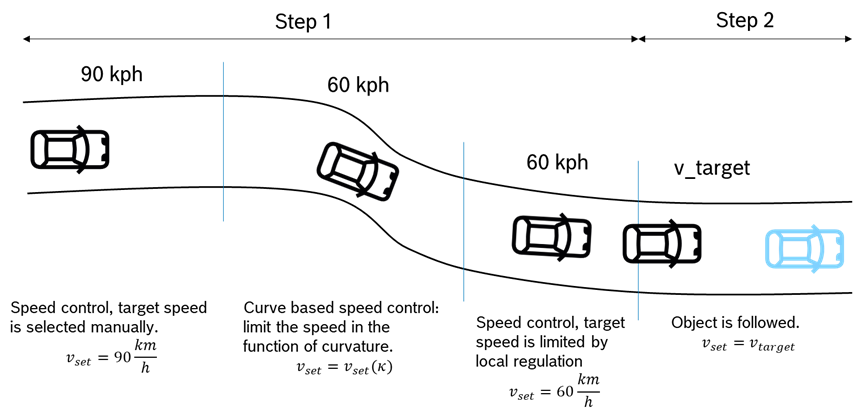
\includegraphics[width=0.8\textwidth]{lon_sa.png}}
    \caption{Function illustration, both step 1 and step 2 functionality.}
    \label{fig:lon_sa}
\end{figure}
\subsection{Longitudinal Emergency Function}
Functionality: vehicle or delegated sensors provide information about static / dynamic objects. The function decides proper strategy to stop the vehicle 
(and where to stop it). Then, this strategy is accomplished by applying proper braking force. Function use cases are shown in Figure \ref{fig:lon_em}.
Operation range: $0.0 \le v_x \le 150.0 kph$.
\begin{figure}[h]
    %\captionsetup{justification=raggedleft}
    \center{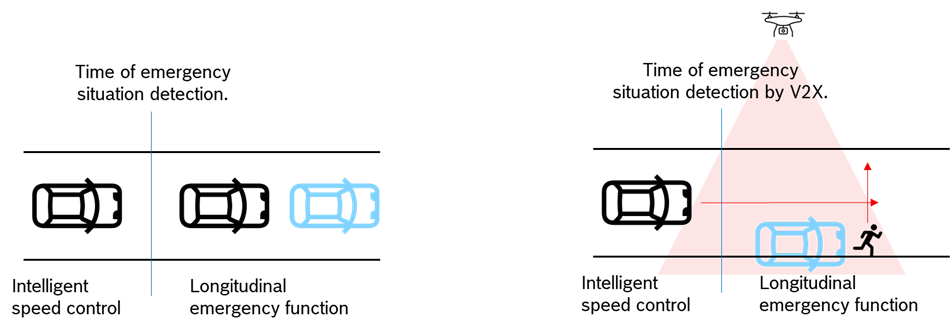
\includegraphics[width=0.8\textwidth]{lon_em.png}}
    \caption{Longitudinal emergency use cases from vehicle sensors and infrastructure sensors.}
    \label{fig:lon_em}
\end{figure}

\subsection{Lane Follow}
\begin{itemize}
    \item Step 1 functionality: vehicle is running in a lane, which is bounded by lane edges (markers or only the edge of the drivable surface) and the vehicle follows the centerline of the lane (or externally defined local trajectory). Operation range: $a_{y,max}=5 m/s^2$ , $0.0 kph \le v_x \le 150.0 kph$, $\sigma_{e_y}^2 \le 0.1 m$.
	\item Step 2 functionality: Drivable corridor is shifted due to e.g., temporarily shifted road works, which is bounded by 3D obstacles like cones, walls...etc. Vehicle (with lower dynamics) can still navigate through this drivable corridors. Operation range: $a_{y,max}=3 m/s^2$ , $0.0 kph \le v_x \le 110.0 kph$, $\sigma_{e_y)}^2 \le 0.1 m$.
\end{itemize}
\begin{figure}[h]
    %\captionsetup{justification=raggedleft}
    \center{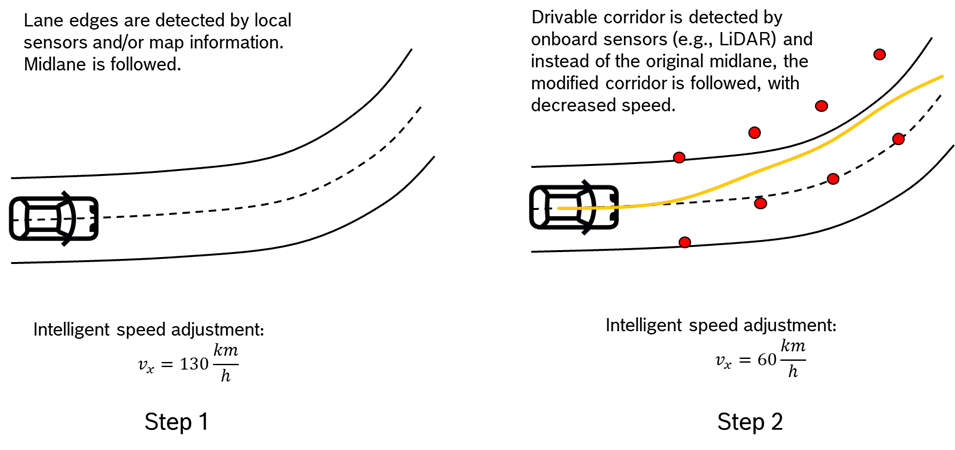
\includegraphics[width=0.8\textwidth]{lat_comf.png}}
    \caption{Lane follow functionality steps and covered operation.}
    \label{fig:lat_comf}
\end{figure}

\section{Architecture Specification} \label{arch_spec}
\subsection{Comprehensive notes}
The architecture is defined based on the E2E function specifications. There are two main concepts that must be considered at all time:
\begin{itemize}
    \item fulfill E2E function requirements with the least architecture components,
    \item re-use Autoware components where possible, but keeping its number (or number/function) as low as possible.
\end{itemize}
Therefore, the work model shown in Figure \ref{fig:cycle} is strongly recommended.
\begin{figure}[h]
    %\captionsetup{justification=raggedleft}
    \center{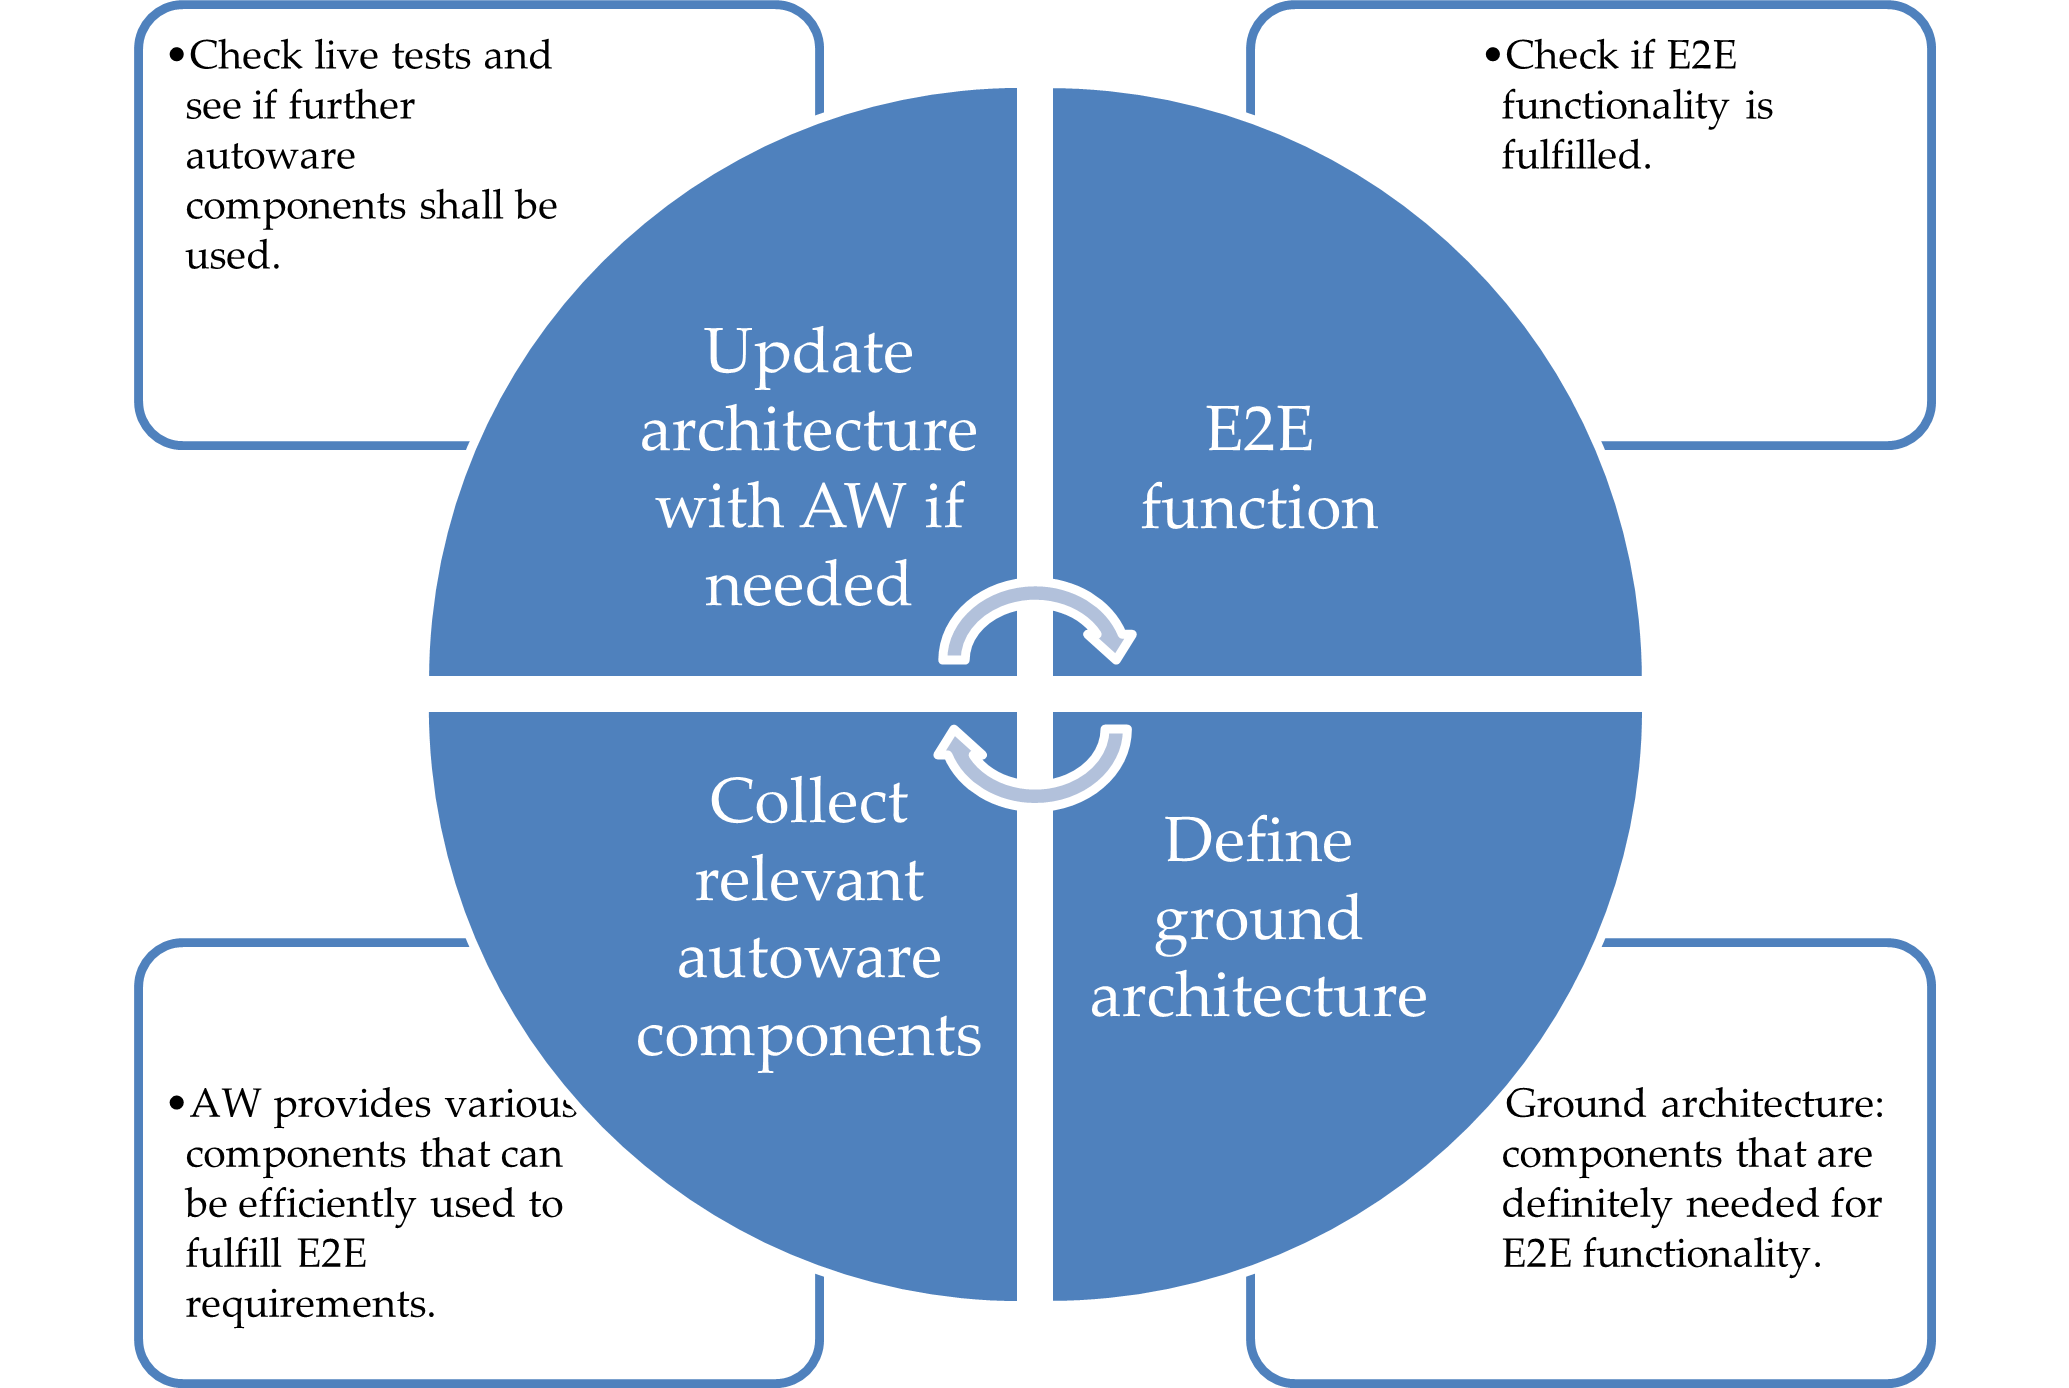
\includegraphics[width=0.8\textwidth]{cycle.png}}
    \caption{Working cycle - proposal}
    \label{fig:cycle}
\end{figure}
This concept may hinder the efficient/reliable planning of tasks regarding architecture definition, but ensures that the above two concepts are respected.

\subsection{General Architecture}
\subsubsection{High-level Black-box architecture}
\begin{figure}[h]
    %\captionsetup{justification=raggedleft}
    \center{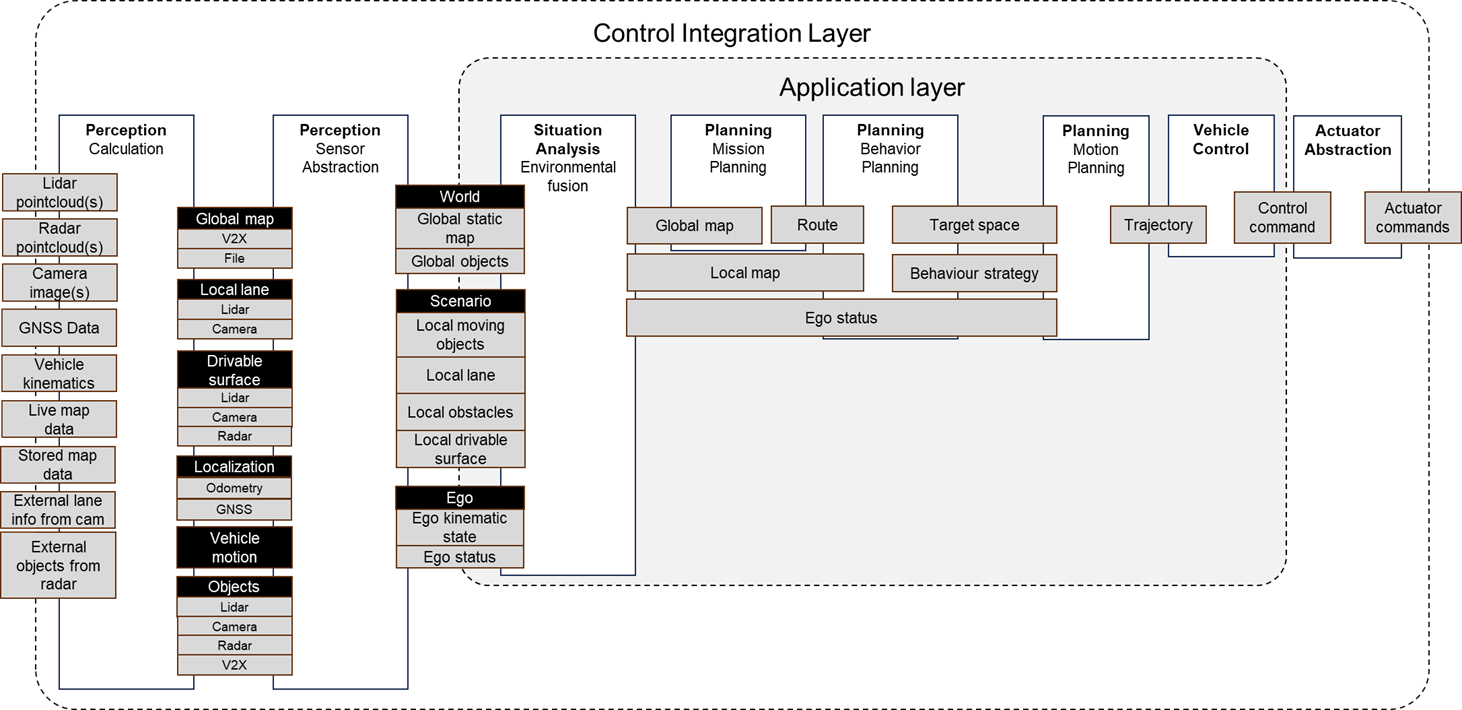
\includegraphics[width=1.0\textwidth]{gen_arch.png}}
    \caption{Black box architecture}
    \label{fig:gen_arch}
\end{figure}
\subsubsection{Gray-box architecture}
\begin{figure}[h]
    %\captionsetup{justification=raggedleft}
    \center{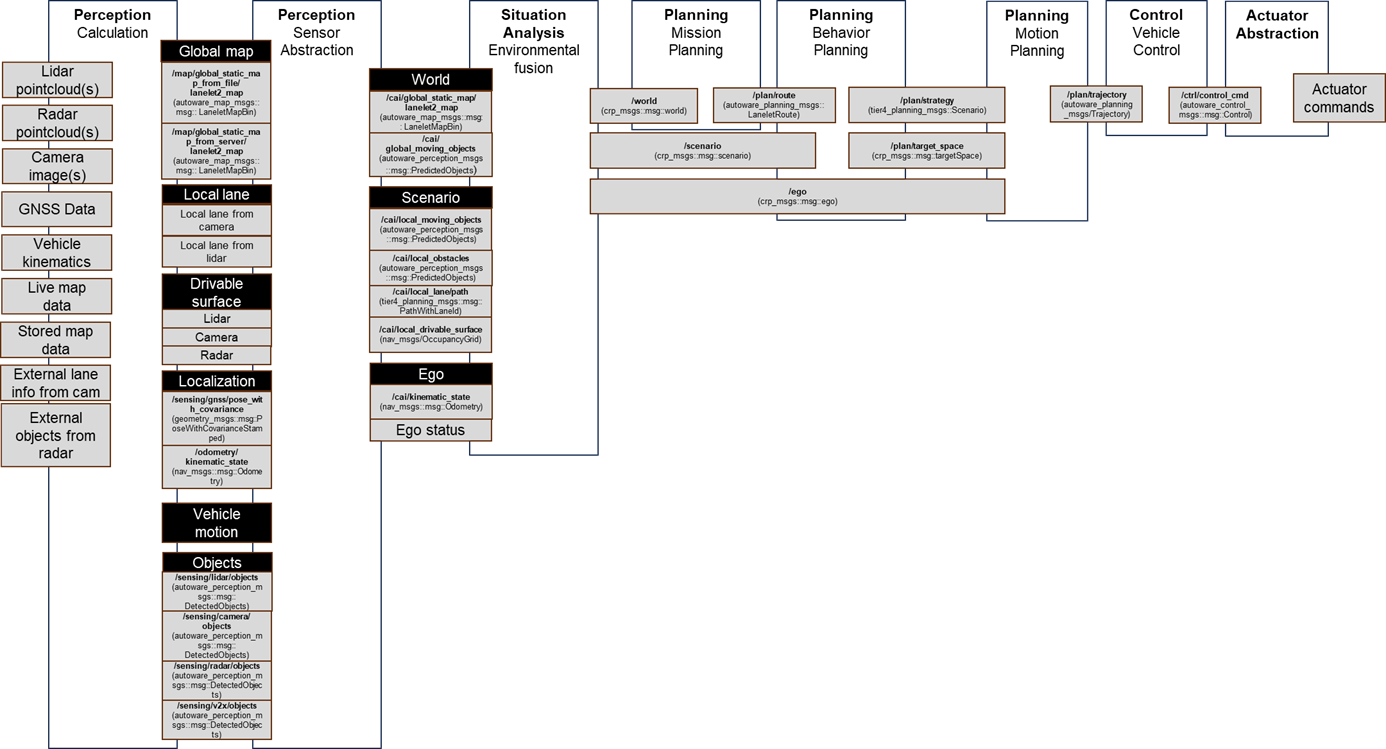
\includegraphics[width=1.0\textwidth]{gray_arch.png}}
    \caption{Gray box architecture.}
    \label{fig:gray_arch}
\end{figure}
\subsubsection{Functional (ROS2) architecture}
\begin{figure}[h]
    %\captionsetup{justification=raggedleft}
    \center{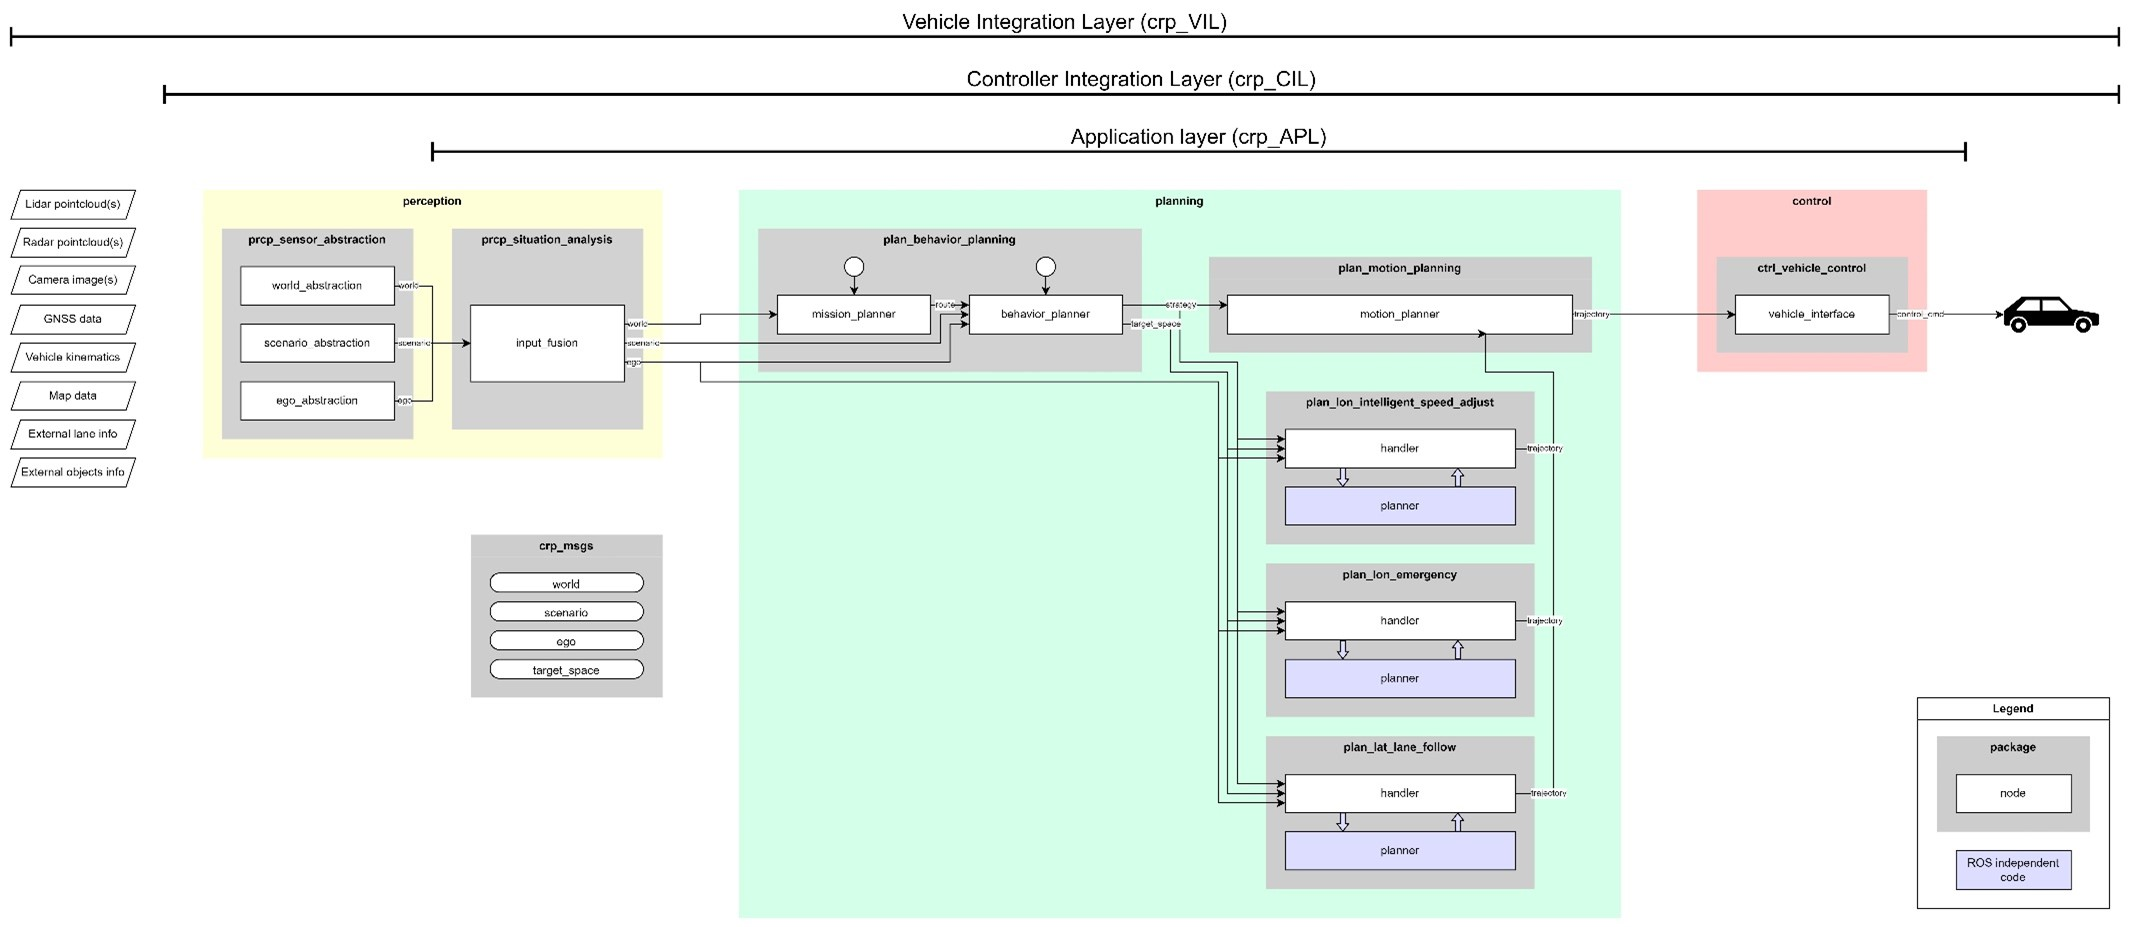
\includegraphics[width=1.0\textwidth]{func_arch.jpg}}
    \caption{Functional architecture}
    \label{fig:fun_arch}
\end{figure}

\subsection{Function Architecture Specification}
\subsubsection{Intelligent Speed Adjustment}
Step 1 architecture is shown in Figure \ref{fig:sa_step1}.
\begin{figure}[h]
    %\captionsetup{justification=raggedleft}
    \center{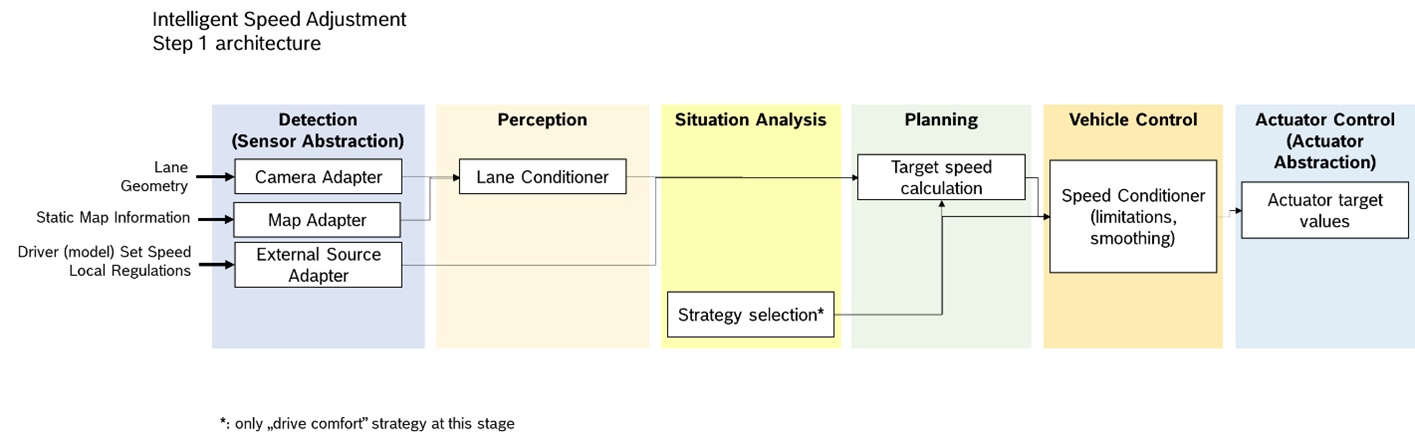
\includegraphics[width=0.8\textwidth]{gen_arch_sa_step1.png}}
    \caption{Architecture components of step 1 functionality of ISA}
    \label{fig:sa_step1}
\end{figure}
Note: even if we only control the vehicle longitudinally, the lateral path shall be filled with dummy values. Idea: add a straight line with no offset. Later, it must be solved that the vehicle is longitudinally controlled by the system, but laterally by the driver.
\newline Step 2 architecture is shown in Figure \ref{fig:sa_step2}.
\begin{figure}[h]
    %\captionsetup{justification=raggedleft}
    \center{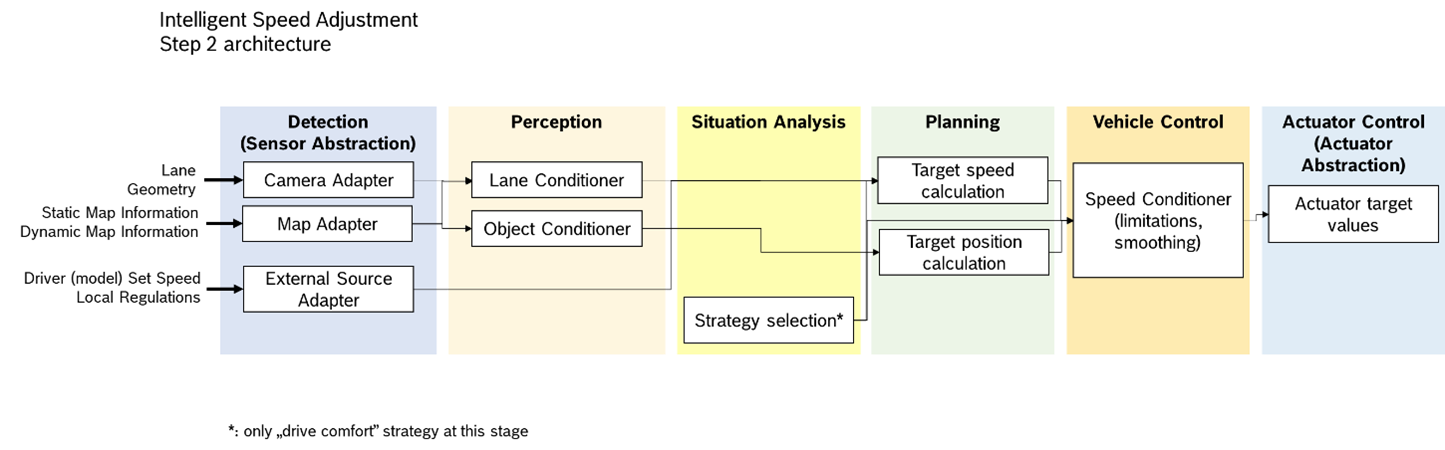
\includegraphics[width=0.8\textwidth]{gen_arch_sa_step2.png}}
    \caption{Architecture components of step 2 functionality of ISA}
    \label{fig:sa_step2}
\end{figure}

\subsubsection{Longitudinal emergency function}
Based on distributed sensor data calculate the trigger of the emergency scenario. Corresponding architecture is shown in Figure \ref{fig:em_step1}.
\begin{figure}[h]
    %\captionsetup{justification=raggedleft}
    \center{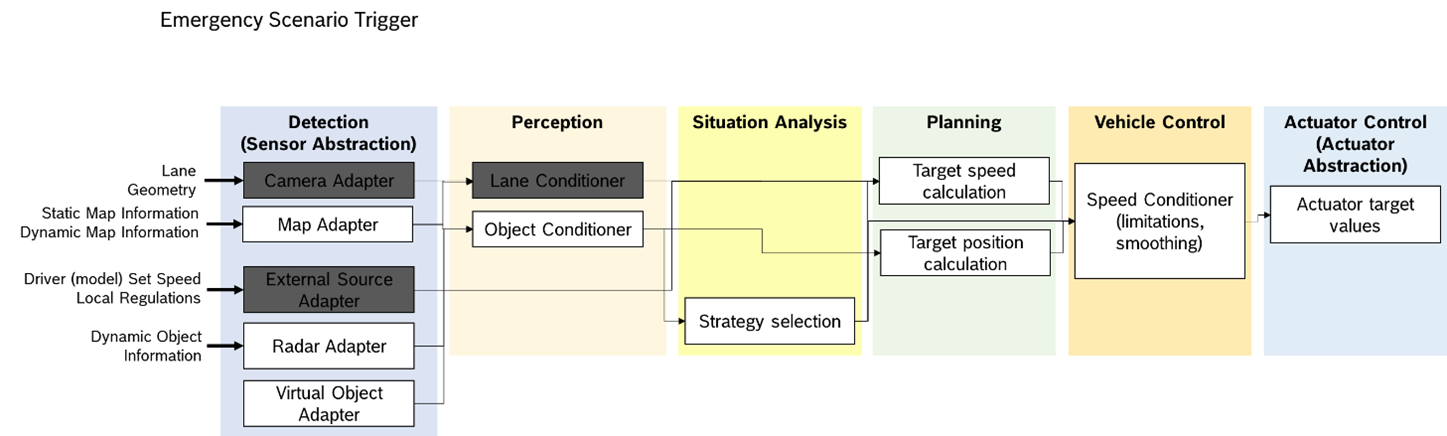
\includegraphics[width=0.8\textwidth]{gen_arch_em.png}}
    \caption{Architecture components of step 1 longitudinal emergency function.}
    \label{fig:em_step1}
\end{figure}

\subsubsection{Lane Follow}
Lane follow functional architecture is shown in Figure \ref{fig:lat_step1}.
\begin{figure}[h]
    %\captionsetup{justification=raggedleft}
    \center{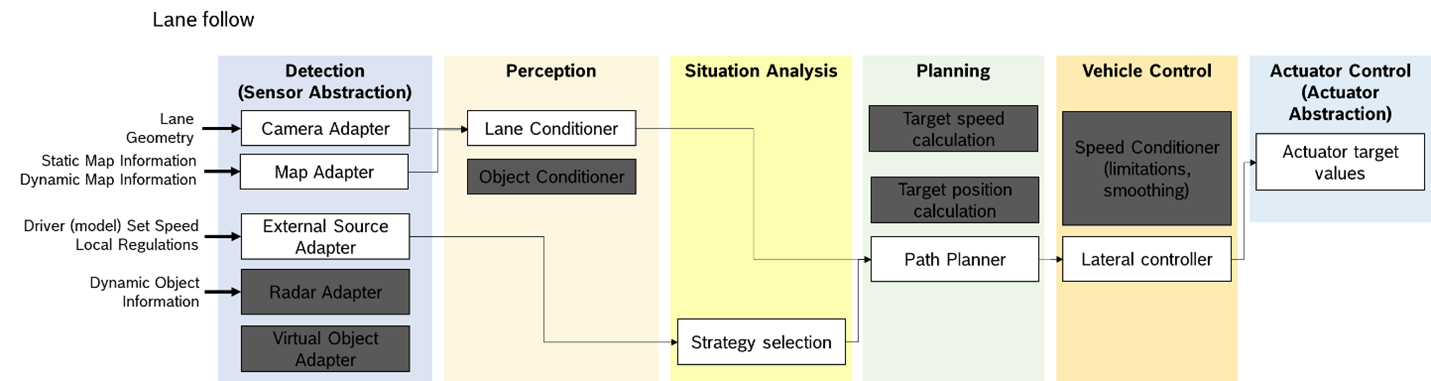
\includegraphics[width=0.8\textwidth]{gen_arch_lat_step1.png}}
    \caption{Architecture components of step 1 functionality of LF (lane follower) without behaviour layer.}
    \label{fig:lat_step1}
\end{figure}
Lane follow architecture consists of new components of path planner, that takes geometry information of the road, and plans a smooth (drivable) path, 
which is then handed over to the lateral controller component. This controller controls only the lateral movement of the vehicle, producing output to the 
actuator control (i.e., steering angle).
Note: route input comes from mission planner, which is currently not part of the architecture. During integration process, it may be extended.
Step 2 architecture is shown in Figure \ref{fig:lat_step2}.
\begin{figure}[h]
    %\captionsetup{justification=raggedleft}
    \center{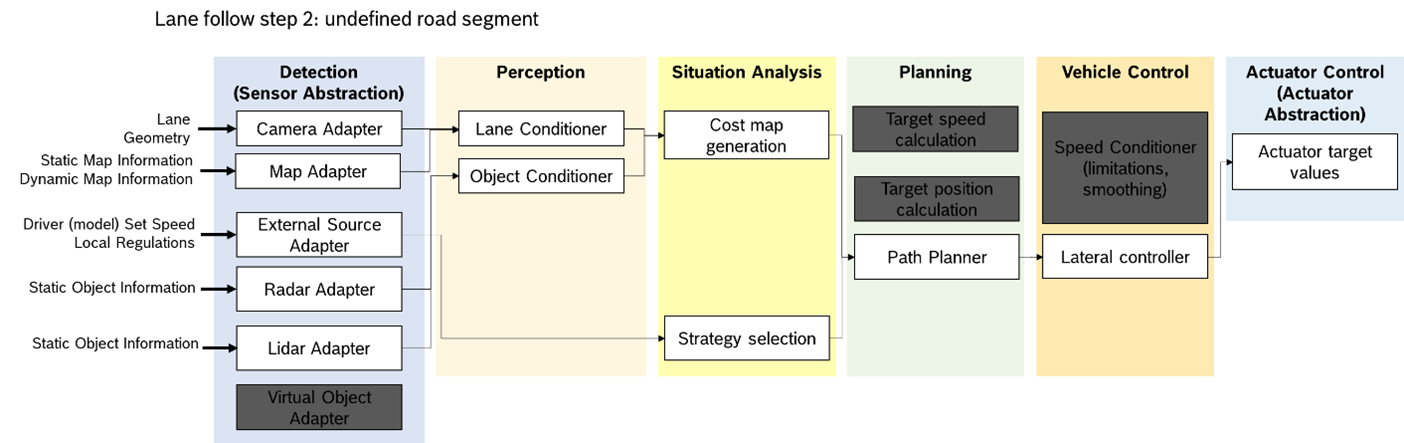
\includegraphics[width=0.8\textwidth]{gen_arch_lat_step2.png}}
    \caption{Architecture components of step 2 functionality of LF (lane follower) without behaviour layer.}
    \label{fig:lat_step2}
\end{figure}

\section{Message Definitions} \label{message_definitions}
\subsection{CRP messages}
\subsubsection{crp\_msgs/msg/scenario}
This interface holds information of four main types:
\begin{itemize}
    \item local moving objects: highest layer which is associated with other objects that move around the ego vehicle, such as other vehicles, pedestrians, animals...etc.
    \item local obstacles: static items that are located around the ego vehicle. 
    \item local lanes: the lanes that are mainly marked by painted markers and form the static driving corridors. 
    \item local drivable surface: the most indefinite representation of the local environment, in the form of a generic occupancy grid.
\end{itemize}
This interface type (in contrast to globally defined 'world' interface) must contain data with as high accuracy as possible.
Message definition:
\begin{lstlisting}
    std_msgs/Header header

    autoware_perception_msgs/PredictedObject[] local_moving_objects
    autoware_perception_msgs/PredictedObject[] local_obstacles
    tier4_planning_msgs/PathWithLaneId[] lanes
    // traffic rules information to be added
    nav_msgs/OccupancyGrid free_space
    std_msgs/Float32 maximum_speed
\end{lstlisting}
Note: the traffic rules collect all types of information that are coming from the static rules and can impact the selected bahviour. These are like:
\begin{itemize}
    \item stop lines (stop signs and lines)
    \item speed limitation
    \item traffic light information (semi-static)...etc.
\end{itemize}
\begin{figure}[h]
    %\captionsetup{justification=raggedleft}
    \center{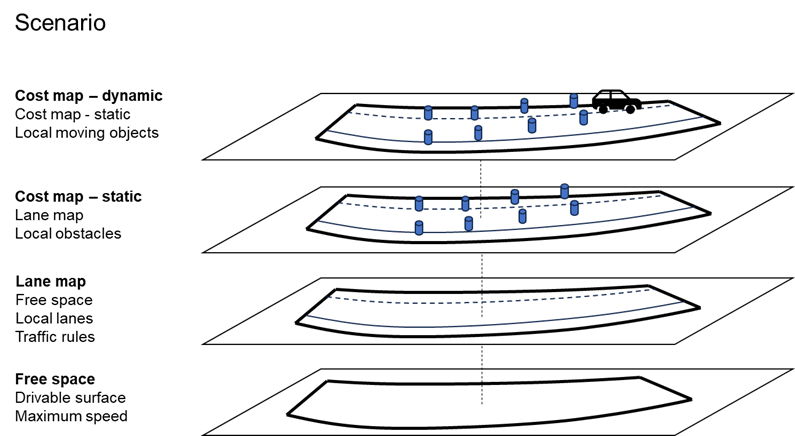
\includegraphics[width=0.8\textwidth]{scenario.png}}
    \caption{Illustration of the scenario layers.}
    \label{fig:scenario}
\end{figure}

\subsubsection{crp\_msgs/msg/world}

\subsubsection{crp\_msgs/msg/ego}
This interface contains every relevant information about the ego vehicle:
\begin{itemize}
    \item pose: position, orientations and uncertainty
    \item velocity: linear and angular
    \item acceleration: linear and angular
    \item wheel angle
\end{itemize}
Message definition:
\begin{lstlisting}
    std_msgs/Header header

    geometry_msgs/PoseWithCovariance pose
    geometry_msgs/TwistWithCovariance twist
    geometry_msgs/AccelWithCovariance accel
    float32 wheel_angle
\end{lstlisting}

\subsection{Tier4 messages in use}
\subsubsection{Path}
This is a tier4 autoware message extension, with the following definition:
\begin{lstlisting}
    std_msgs/Header header

    tier4_planning_msgs/PathPoint[] points
    nav_msgs/OccupancyGrid drivable_area
\end{lstlisting}

\subsubsection{Path point}
\begin{lstlisting}
    uint8 REFERENCE=0
    uint8 FIXED=1
    geometry_msgs/Pose pose
    geometry_msgs/Twist twist
    uint8 type
\end{lstlisting}

\subsubsection{Trajectory}
\begin{lstlisting}
    std_msgs/Header header
    tier4_planning_msgs/TrajectoryPoint[] points
\end{lstlisting}

\subsubsection{Trajectory point}
\begin{lstlisting}
    geometry_msgs/Pose pose
    geometry_msgs/Twist twist
    geometry_msgs/Accel accel
\end{lstlisting}

\section{Using the Platform} \label{using_platform}
\subsection{Installation (source)}
Create workspace and clone the repository:
\begin{lstlisting}
    mkdir -p crp_ws/src
    cd crp_ws/src
    git clone https://github.com/jkk-research/CooperativeResearchPlatform.git --recurse-submodules
\end{lstlisting}
Install dependencies and build the workspace:
\begin{lstlisting}
    cd ..
    rosdep install --from-paths src --ignore-src -y
    colcon build --symlink-install
\end{lstlisting}

\subsection{Using it in a docker container}
\subsubsection{Docker container}
The platform can be used in a docker container. The docker is available here: https://hub.docker.com/repository/docker/anonymdavid/crp/general
\subsubsection{Building the docker}
Alternatively the autoware docker can be built using the script inside the autoware repository. The docker container is built on top of the autoware docker (ghcr.io/autowarefoundation/autoware:latest-devel-cuda). Autoware and CRP should be built for the same platform type (amd64/arm64).
\newline
The container can be build to ARM64 platform:
\begin{lstlisting}
    cd CooperativeResearchPlatform
    ./docker/build_arm64.sh
\end{lstlisting}
\subsubsection{Running the docker}
The docker can be run with the following command:
\begin{lstlisting}
    docker run -it --rm --network host --ipc host --pid host --device /dev/leaf0 --device /dev/leaf1 crp_arm64:latest
\end{lstlisting}
This way the docker shares the network with the host and has access to the kvaser CAN device.

\section{Coding rules} \label{sec:coding_rules}
\subsection{Naming convention}
\begin{itemize}
    \item Use camel case everywhere if not stated otherwise - example: \emph{latLaneFollow}
    \item Classes and structs should start with upper case letter - example: \emph{MotionHandler}
    \item Methods should be camel case (starting with small case) - example: \emph{scenarioCallback}
    \item Method arguments have no prefix/suffix, they must be given with camel case - example: \emph{plannerInput}
    \item Constant variables should be all capital letters. Instead of camel case the words should be separated with '\_' - example: \emph{MAX\_SPEED}
    \item In classes all member variables should start with the 'm\_' prefix - example: \emph{m\_vxEgo}
    \item The runtime calibratable parameters should start with the 'p\_' prefix - example: \emph{p\_mainThreshold}
    \item In special cases (e.g., subscribers/publishers) extra name tags can be added with lower case, separated by underscore - example: \emph{m\_sub\_strategy\_}
    \item Pointers should comply with the previous rules but should have a '\_' suffix - example: \emph{m\_sub\_strategy\_}
    \item Namespaces should be fully lower case - example: \emph{crp}
    \item Maximum namespace depth should be 3
    \item File and folder names should be camel case where it is not restricted (e.g. ROS2 naming rules)
\end{itemize}

\subsection{Cplusplus}
\subsubsection{General}
\begin{itemize}
    \item Header and source files should be separated ('include' folder for headers and 'src' folder for source files)
    \item Header files should only contain declarations, the definitions should be in a source file that includes the header
    \item If applicable, include further header files in the main header file, not in the source file (source file (i.e., cpp) should only include its own declaration header)
    \item Functional code should be included in a separate cmake file (with .cmake extension), which is then included in the main CMakeList.txt (this way, cmake file with functional sources is ROS agnostic)
\end{itemize}

\subsubsection{Header files}
Every header file should…
\begin{itemize}
    \item have the '.hpp' extension,
    \item have header guards (\#ifndef, \#define, \#endif) and it should be all capitals,
    \item contain max. one class.
\end{itemize}

\subsubsection{Source files}
Every source file should…
\begin{itemize}
    \item have the “.cpp” extension.
\end{itemize}

\subsection{ROS2}
\subsubsection{Packages}
Non-driver package names should start with and abbreviation of the following categories:
\begin{itemize}
    \item prcp (perception)
    \item plan (planning)
    \item ctrl (control)
\end{itemize}
All dependencies must be set in the package.xml and in the CMakeList.txt.
\newpage

\section{Package documentations}
\subsection{pacmod\_extender}
\subsubsection{Purpose}
The purpose of this package is to extend the default pacmod capabilities on the Lexus vehicle by decoding CAN messages or calculating new data from the inputs. The package is designed to work seamlessly with the already existing pacmod3 system.
\subsubsection{Usage}
The package can be used by running the executable node. This way it uses the default namespace for subscriptions and publishers:
\begin{lstlisting}
    ros2 run pacmod_extender pacmod_extender_node
\end{lstlisting}
The other way is to use the launcher. This launcher is tailored for the Lexus vehicle by giving the executable the necessary namespace to match the other components:
\begin{lstlisting}
    ros2 launch pacmod_extender pacmod_extender.launch.py
\end{lstlisting}

\subsubsection{IO}
Input topics are given in Table \ref{tab:pacmod_input}, outputs are given in Table \ref{tab:pacmod_output}.
\begin{table}[!h]
    \captionsetup{justification=centering}
    \normalsize
        \caption{\label{tab:pacmod_input} Pacmod extender inputs.}
        \begin{tabular}{ | c | c | c |}
            \hline
            \textbf{Data} & \textbf{Message name} & \textbf{Message Type} \\
            \hline
            Raw can data & pacmod\slash can\_tx & can\_msgs\slash msg \slash Frame \\
            \hline
            Vehicle test & vehicle\_status & geometry\_msgs\slash msg\slash TwistStamped \\
            \hline
        \end{tabular}
\end{table}
\begin{table}[!h]
    \captionsetup{justification=centering}
    \normalsize
        \caption{\label{tab:pacmod_output} Pacmod extender output.}
        \begin{tabular}{ | c || c | c |}
            \hline
            \textbf{Data} & \textbf{Message name} & \textbf{Message Type} \\
            \hline
            Linear acceleration & pacmod/linear\_accel\_rpt & pacmod3\_msgs/msg/LinearAccelRpt \\
            \hline
            Calculated yaw rate & pacmod/yaw\_rate\_calc\_rpt & Pacmod3\_msgs/msg/YawRateRpt \\
            \hline
        \end{tabular}
\end{table}
\subsubsection{Inner workings}
The main functionality is the decoding of previously not used CAN messages. The decodings are defined in the PacmodDefinitions class. Every message has a decode method that requires the CAN message as parameter. The message IDs are stored as constants in the class.
The PacmodExtender class is the main class that is executed as a node. It subscribes to the inputs, uses the PacmodDefinitions class to decode the CAN messages and outputs the new messages. The output rate of every message depends on the input frequencies. Every output value is in SI units.
Decodings:
\begin{itemize}
	\item Linear acceleration
	\item longitudinal, lateral, vertical acceleration in m/s
\end{itemize}
Calculations:
\begin{itemize}
	\item Yaw rate $\psi= v_\xi  tan(\frac{\alpha_f}{L_w})$, where $\psi$ is the yaw rate, $\alpha_f$ is the front road-wheel angle and $L_w$ is the wheelbase.
\end{itemize}


\subsection{duro\_gps\_launcher}
\subsubsection{Purpose}
The purpose of this package is to launch the duro GPS driver. The driver is in a separate repository included as a subrepository. It also contains a node (duro\_topic\_converter) that converts the duro GPS topics to the predefined CRP topics.
\subsubsection{Usage}
The package only contains the launcher for the driver. This can be started as follows:
\begin{lstlisting}
    ros2 launch duro_gps_wrapper duro.launch.py
\end{lstlisting}
\subsubsection{Launch parameters}
The parameters of the launcher are given in Table \ref{tab:duro_gps_wrapper}. The default values are set for the Lexus vehicle.
\begin{table}[!h]
    \captionsetup{justification=centering}
    \normalsize
    \caption{\label{tab:duro_gps_wrapper} Duro gps launcher parameters.}
    \begin{tabular}{| l | l | l |}
        \hline
        \textbf{Name} & \textbf{Default value} & \textbf{Description} \\
        \hline
        duro\_namespace  & gps/duro       & Namespace for the Novatel GPS \\
        \hline
        duro\_ip         & 192.168.10.11  & IP address of the Duro GPS \\
        \hline
        duro\_port       & 5555           & Port of the Novatel GPS \\
        \hline
    \end{tabular}
\end{table}


\subsection{novatel\_gps\_launcher}
\subsubsection{Purpose}
The purpose of this package is to launch the novatel GPS driver. The driver is in a separate repository included as a subrepository. It also contains a node (novatel\_topic\_converter) that converts the novatel GPS topics to the predefined CRP topics.
\subsubsection{Usage}
The package only contains the launcher for the driver. This can be started as follows:
\begin{lstlisting}
    ros2 launch novatel_gps_wrapper novatel.launch.py
\end{lstlisting}
\subsubsection{Launch parameters}
The parameters of the launcher are given in Table \ref{tab:novatel_gps_wrapper}. The default values are set for the Nissan leaf vehicle.
\begin{table}[!h]
    \captionsetup{justification=centering}
    \normalsize
    \caption{\label{tab:novatel_gps_wrapper} Novatel gps launcher parameters.}
    \begin{tabular}{| l | l | l |}
        \hline
        \textbf{Name} & \textbf{Default value} & \textbf{Description} \\
        \hline
        novatel\_namespace  & gps/nova          & Namespace for the Novatel GPS \\
        \hline
        novatel\_ip         & 192.168.1.11      & IP address of the Novatel GPS \\
        \hline
        novatel\_port       & 3002              & Port of the Novatel GPS \\
        \hline
        novatel\_imu\_frame & /nissan9/nova/imu & IMU frame id of the Novatel GPS \\
        \hline
        novatel\_frame\_id  & /nissan9/nova/gps & Frame id of the Novatel GPS \\
        \hline
    \end{tabular}
\end{table}


\subsection{lanelet\_handler}
\subsubsection{Purpose}
The purpose of this package is to load and publish a lanelet2 map to a specified topic using the autoware lanelet2 library.
\subsubsection{Usage}
The package can be used by the provided launcher:
\begin{lstlisting}
    ros2 launch lanelet_handler laneletFileLoader.launch.py
\end{lstlisting}
\subsubsection{Launch parameters}
Launch parameters are given in Table \ref{tab:lanelet_handler}.
\begin{table}[!h]
    \centering
    \captionsetup{justification=centering}
    \normalsize
    \caption{\label{tab:lanelet_handler} Launch parameters.}
    \begin{tabular}{| l | l | l |}
        \hline
        \textbf{Name} & \textbf{Default value} & \textbf{Description} \\
        \hline
        map\_file\_path           &                                       & Path to the lanelet2 map file \\
        \hline
        map\_output\_topic        & /map/global\_static\_map\_from\_file/ & Output topic for the map binary \\
                                  & lanelet2\_map                         &  \\
        \hline
        map\_frame\_id            & map                                   & Frame id of the lanelet2 map \\
        \hline
        map\_visualization\_topic & /map/global\_static\_map\_from\_file/ & Frame id of the lanelet2 map \\
                                  & lanelet2\_map\_visualization          &  \\
        \hline
    \end{tabular}
\end{table}


\subsection{mcap\_rec}
\subsubsection{Purpose}
This package contains scipts for recording all the necessary topics of the project.
\subsubsection{Usage}
The package can be used by the provided launchers:
\begin{lstlisting}
    ros2 launch mcap_rec recordLexus.launch.py tag:=name_of_the_recording
\end{lstlisting}
\subsubsection{Recorded params}
Each launcher has a different preset for which topics to record. The recorded topics are defined in the etc folder in txt files.


\subsection{nissan\_can\_driver}
\subsubsection{Purpose}
The purpose of this package is to publish the vehicle status (speed, steering) to topics and receive control commands from topics to control the vehicle.
\subsubsection{Usage}
The package can be used by the provided launcher:
\begin{lstlisting}
    ros2 launch nissan_can_driver can_driver_kvaser.launch.py
\end{lstlisting}
In the current implementation a kvaser device with 2 channels is used for the communication. On the first channel the CAN data is received from the vehicle and on the second channel the control commands are sent to the controllers.
\subsubsection{Launch parameters}
Launch parameters are given in Table \ref{tab:nissan_can_driver_params}.
\begin{table}[!h]
    \centering
    \captionsetup{justification=centering}
    \normalsize
    \caption{\label{tab:nissan_can_driver_params} Launch parameters.}
    \begin{tabular}{| l | l | l |}
        \hline
        \textbf{Name} & \textbf{Default value} & \textbf{Description} \\
        \hline
        autoware\_control\_input & True  & Whether to use autoware or standard type \\
                                 &       & input message for control \\
        \hline
        kvaser\_hardware\_id     & 11162 & HW ID of the kvaser device used for CAN communication \\
        \hline
    \end{tabular}
\end{table}
\subsubsection{IO}
Input topics are given in Table \ref{tab:nissan_can_driver_inputs}.
\begin{table}[!h]
    \centering
    \captionsetup{justification=centering}
    \normalsize
    \caption{\label{tab:nissan_can_driver_inputs} Launch parameters.}
    \begin{tabular}{| l | l | l |}
        \hline
        \textbf{Name} & \textbf{Message type} & \textbf{Description} \\
        \hline
        /ctrl/control\_cmd  & autoware\_control\_msgs/msg/Control & Control input topic if \textit{autoware\_control\_input}  \\
                            &                                     & is set to true                                            \\
                            &                                     & Contains speed and steering commands                      \\
        \hline
        /ctrl/speed\_cmd    & std\_msgs/msg/Float32                & Control input topic if \textit{autoware\_control\_input} \\
                            &                                     & is set to true                                            \\
                            &                                     & Contains speed command (m/s)                              \\
        \hline
        /ctrl/steering\_cmd & std\_msgs/msg/Float32                & Control input topic if \textit{autoware\_control\_input} \\
                            &                                     & is set to true                                            \\
                            &                                     & Contains steering command (tire angle, rad)               \\
        \hline
    \end{tabular}
\end{table}

\section{Map Creation}
\subsection{Data Process}
To create lane maps, the following devices were used in a single vehicle:
\begin{itemize}
    \item Bosch MPC2.0 video camera - detecting lane edge markings \cite{mpc25},
    \item ADMA Gen3 GNSS system with RTK service - for accurate localization \cite{adma}.
\end{itemize}
According to the datasheet of the devices, the camera estimates lane marking centerpoint position compared to the vehicle rear axis with an accuracy of $2 cm$, 
assuming confidence of at least $75\%$. The confidence value is also provided by the camera and measured during our test drives. In the data process phase 
measurement points that have lower confidence than this threshold are neglected. Then, the points of the lane edges and centerlines are calculated. 
The camera returns various parameters of the lane edges. These are the following:
\begin{itemize}
    \item $d$ - lateral position of the lane edge(s) in the ego vehicle frame (note: the ego vehicle frame is aligned with the middle point of the rear axle),
    \item $\Theta$ - orientation offset to the lane edge(s),
    \item $\kappa = \frac{1}{R}$ - curvature of the lane edge(s).
\end{itemize}
All quantities are calculated at $x=0$ local coordinate. An illustration of the parameters is shown in Figure \ref{fig:lanegeometry}.
\begin{figure}[h]
    %\captionsetup{justification=raggedleft}
    \center{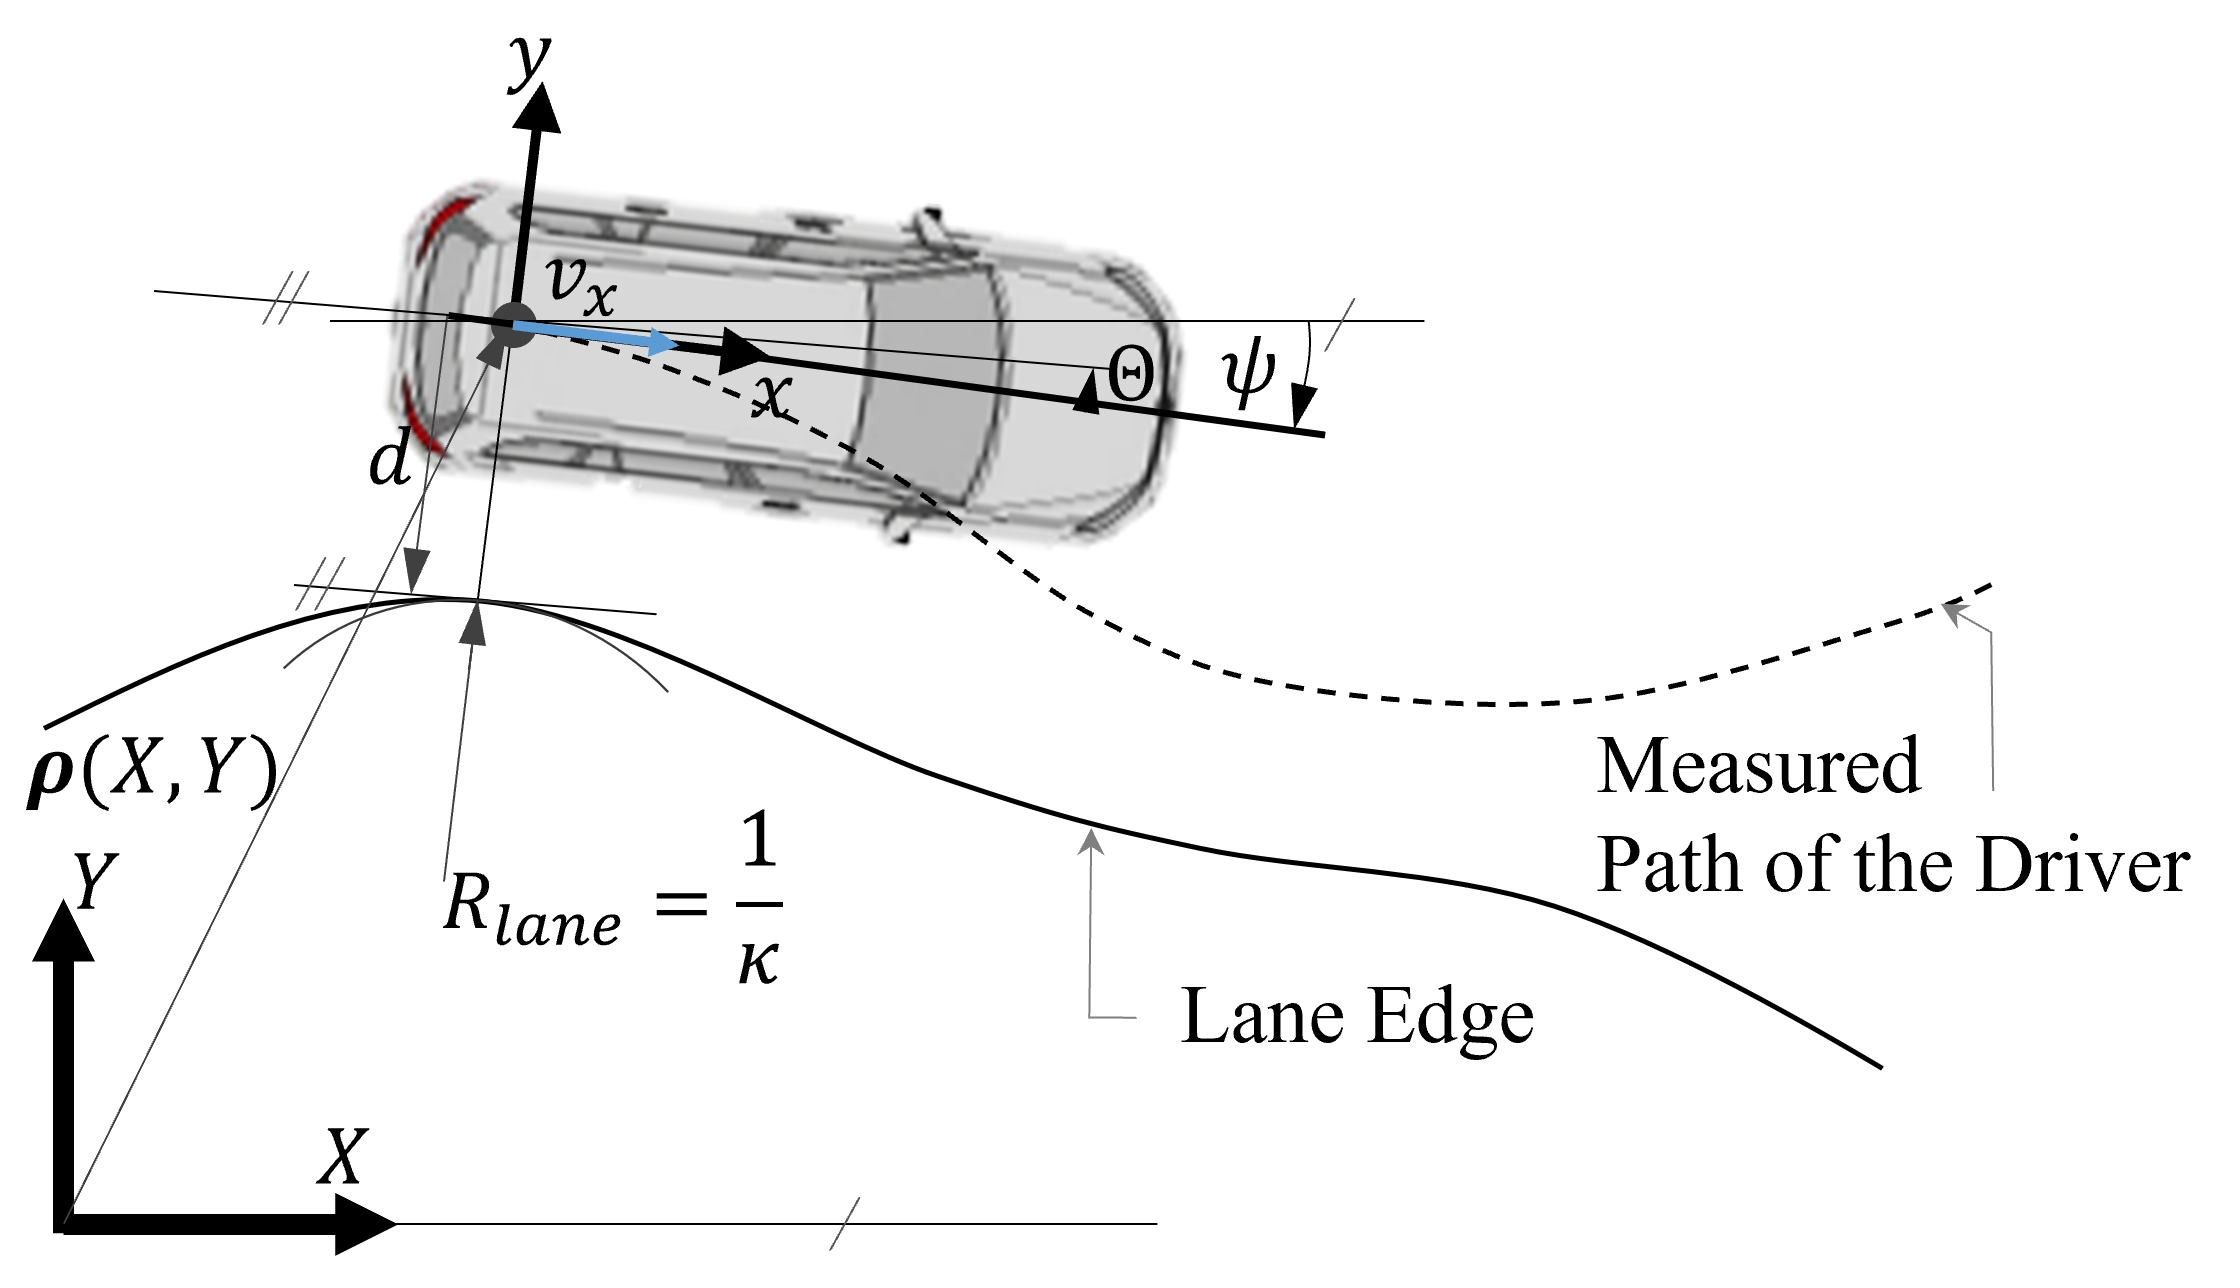
\includegraphics[width=0.6\textwidth]{mapPub/lanegeometry.png}}
    \caption{The lane geometry relations in the ego vehicle frame.}
    \label{fig:lanegeometry}
\end{figure}
Knowing the pose of the ego vehicle, i.e., $\boldsymbol{P}_{ego} = \begin{bmatrix}
    \boldsymbol{\rho}(X,Y) & \Psi
\end{bmatrix}$ the global (UTM) position and orientation of the vehicle, the all-time lane edge 
point at $x=0$ local coordinate can be calculated from $\boldsymbol{P}_{ego}$ and $d(x=0)$, with the following simple 2D transformation equations:
\begin{align} \label{eq:2DTransform}
    X_{lane}(t) = X(t) - sin(\Psi(t))d(t) \\
    Y_{lane}(t) = Y(t) + cos(\Psi(t))d(t)
\end{align}
The camera used in the current study can detect the lane edges of the ego lane, therefore there are $d_{left}(t)$ and $d_{right}(t)$. The lateral distance to the 
centerline of the lane is calculated as the average of the left and right lane edge distance values, namely: $d_{center}(t) = 0.5*(d_{left}(t)+d_{right}(t))$.
\begin{figure}[h]
    %\captionsetup{justification=raggedleft}
    \center{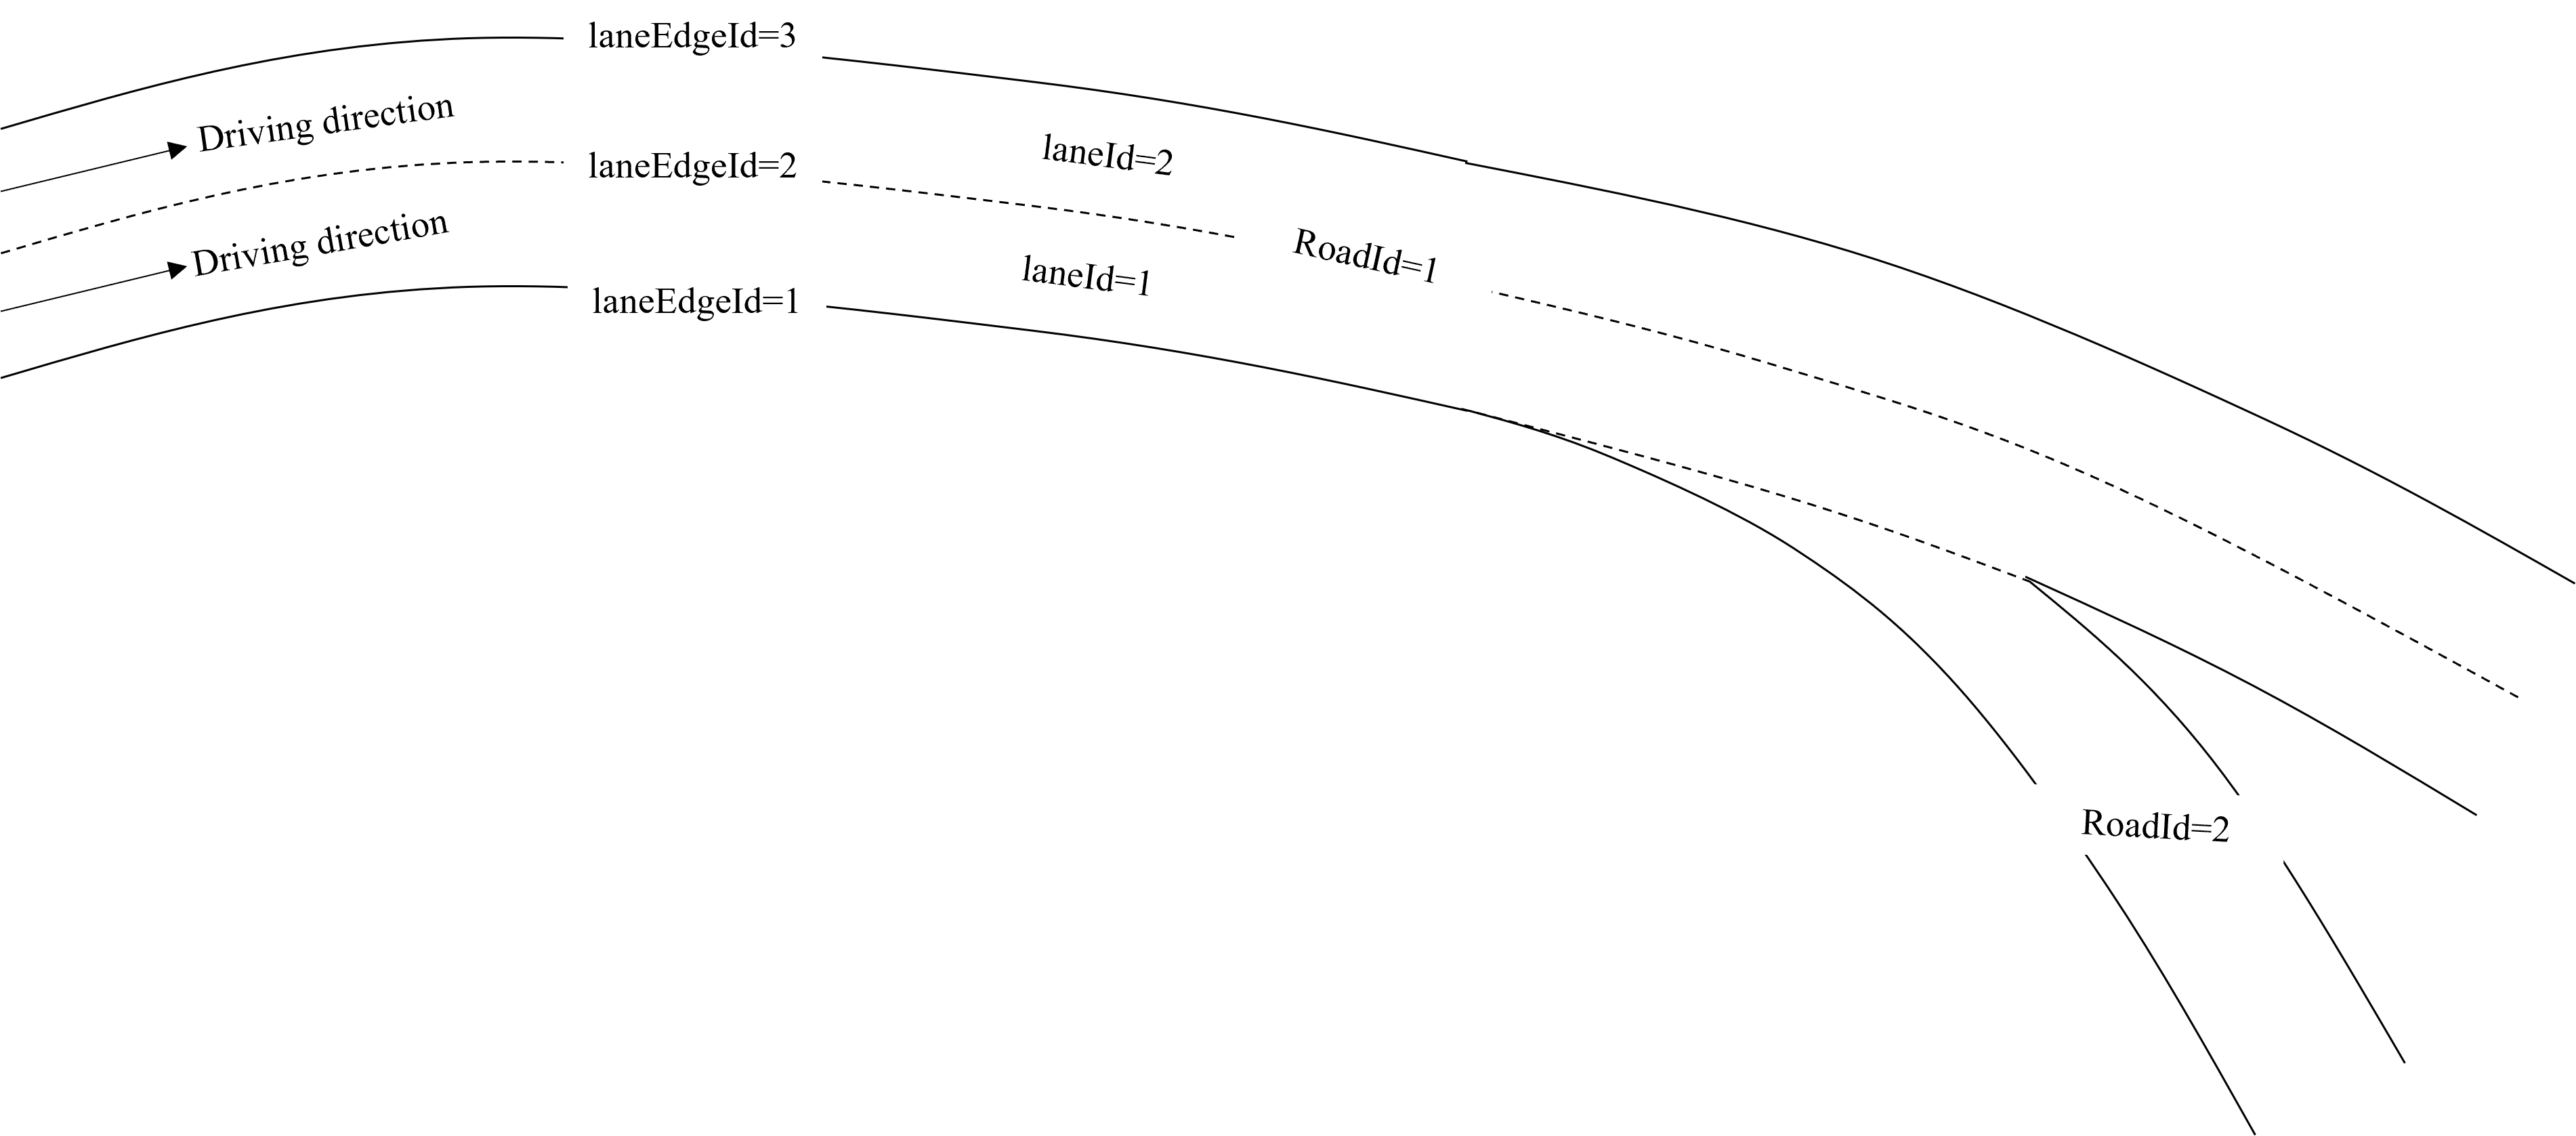
\includegraphics[width=1.0\textwidth]{mapPub/idInterpretation.png}}
    \caption{Interpretation of the lane identification numbers - illustration only.}
    \label{fig:idInterpretation}
\end{figure}
\newline
After the lane marking points are processed, they are saved to a compact structure. In this structure, each lane edge marking, as well as the centerline are stored 
separately. 
\begin{figure}[h]
    %\captionsetup{justification=raggedleft}
    \center{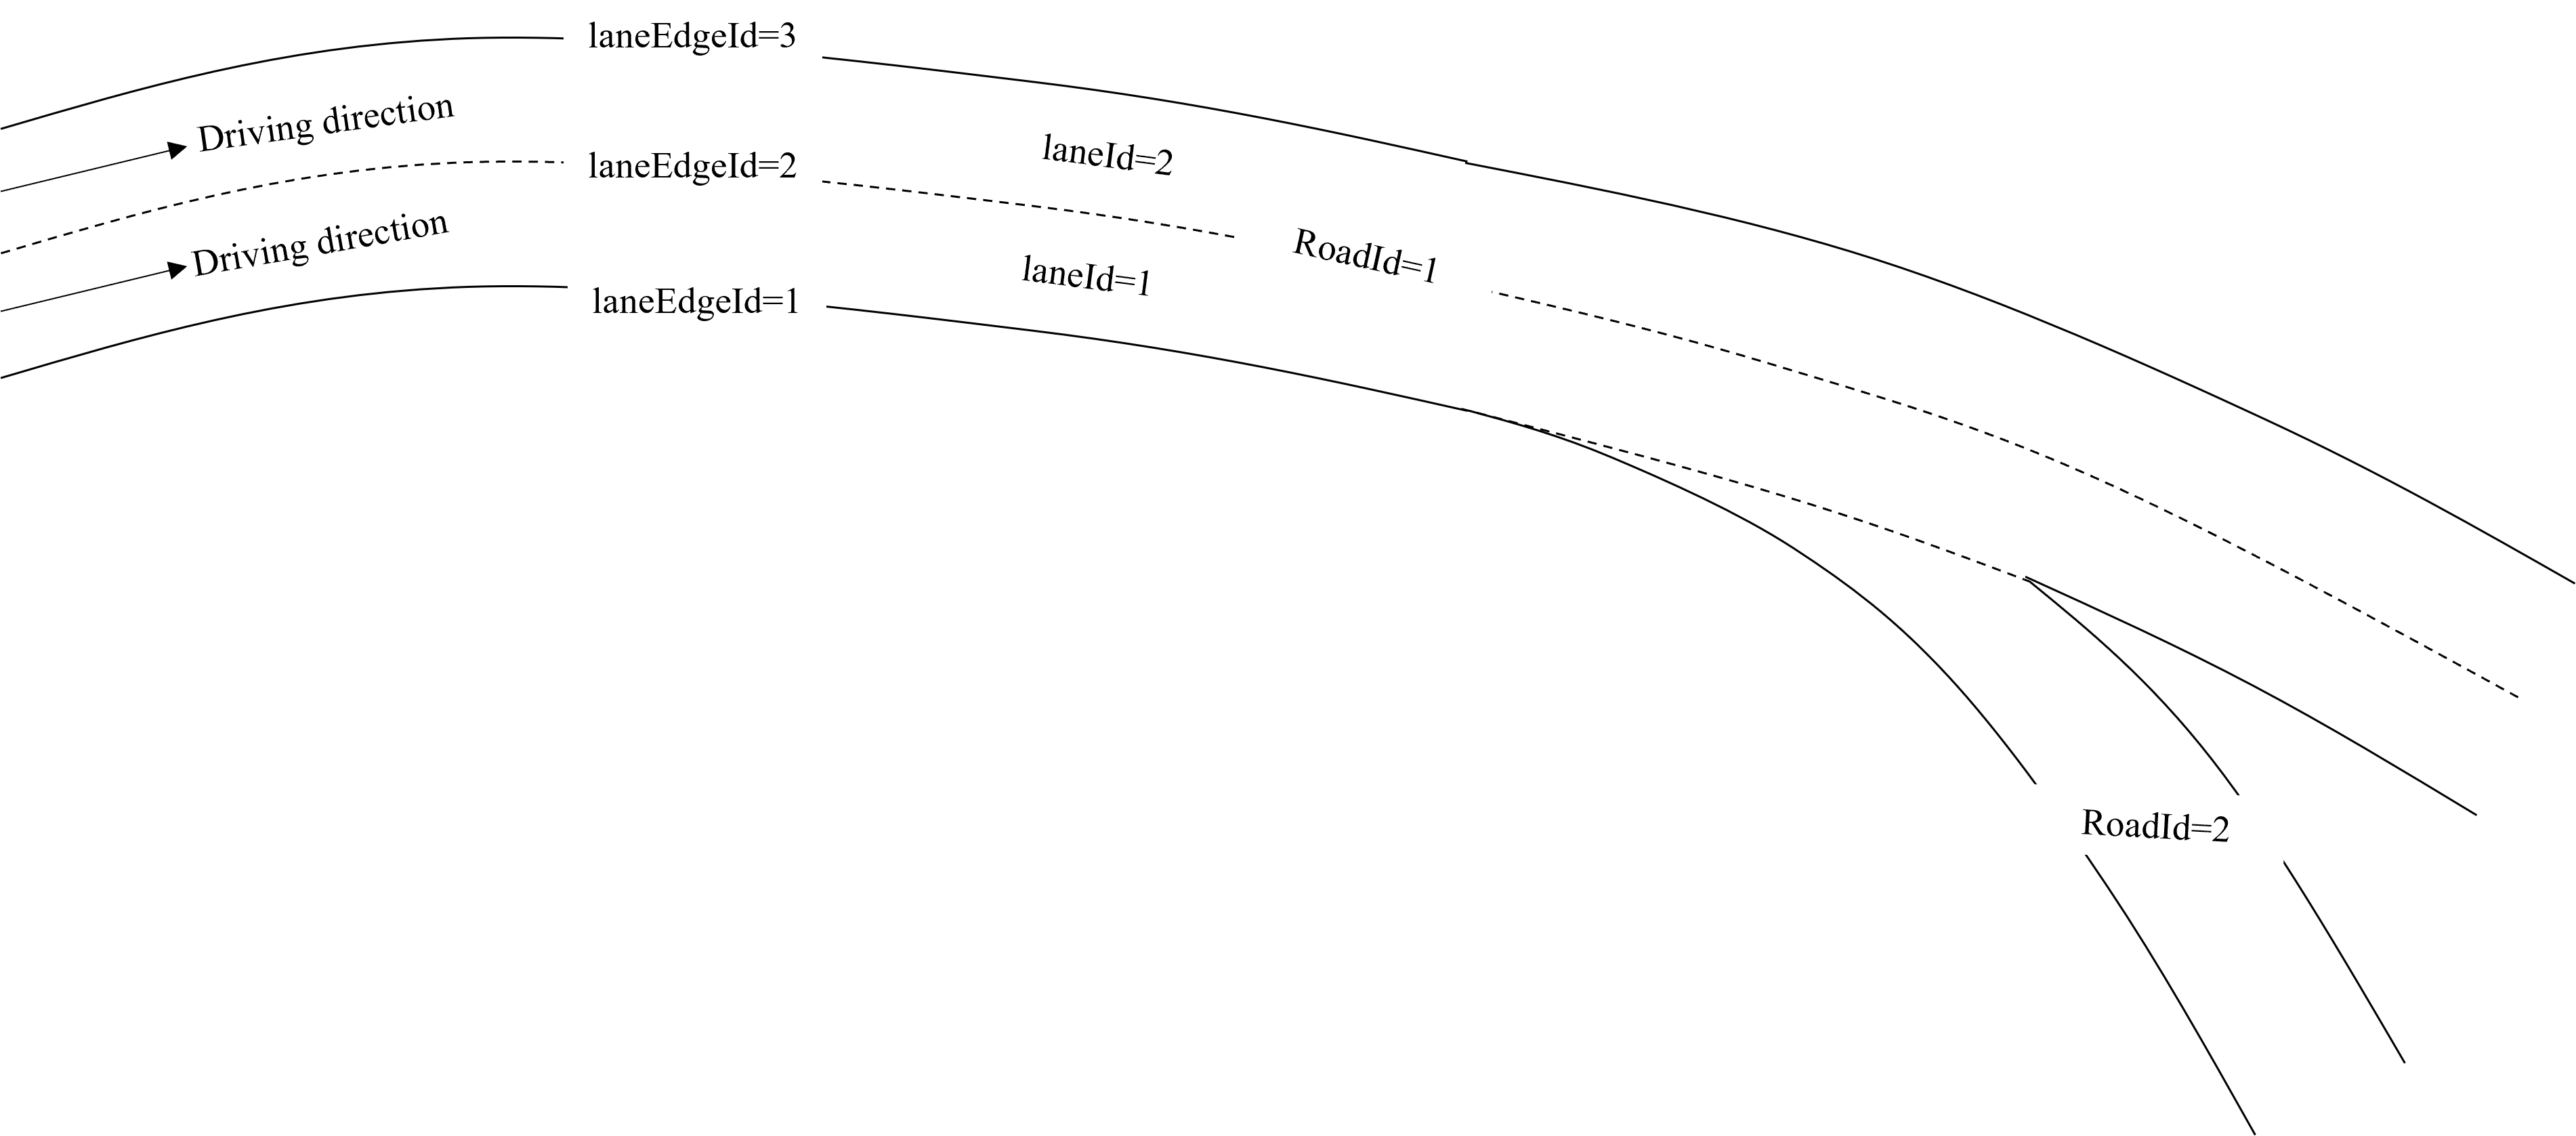
\includegraphics[width=1.0\textwidth]{mapPub/idInterpretation.png}}
    \caption{Interpretation of the lane identification numbers - illustration only.}
    \label{fig:idInterpretation}
\end{figure}
\newline
\newline
\fbox{Note: the steps given in this subsection are implemented in \emph{dataPreprocess.m}}

\subsection{Algorithm steps}
By this point, a well conditioned structure of the lane edges and centerlines are produced. The preprocess steps are summarized as follows:
\begin{enumerate}
    \item Read raw measurement files and do the name standardization,
    \item pre-filtering unreliable measurement points either due to camera maldetection or DGPS inaccuracies,
    \item apply 2D transformation to calculate line points of lane edges and the centerlines,
    \item match the road, lanes and lane edges to predefined identification numbers.
\end{enumerate}
Out of this list, the first three steps can be done without any issues. However, the last step is difficult with no prior knowledge. E.g., how shall we know which road 
the vehicle is on? By knowing the road ID, how can we decide which lane the vehicle travels in (especially valid for multi-lane roads, such as highways)?
To overcome this issue, we propose the following two-step approach:
\begin{itemize}
    \item Step 1: \textbf{referencing phase}. In this phase we create reference lanelets that contain all ID information and a bounding box around each lane lines. The bounding box approach allows a certain deviation from the reference line but still ensures accurate mapping of the new meausurement to the existing lanes. The source of the reference lanes is discussed later.
    \item Step 2: \textbf{accurate phase}. In this phase we read new measurements from the raw files, and match the lanes in it to the reference lines. Once this is done, the stored reference line is recalculated and made more accurate with the information held by the new measurement. The assumption is the more occurance of one lane line the more accurate the reference line.
\end{itemize}
The two-phase approach is also illustrated in Figure \ref{fig:twoPhaseApproach}. The reference file can come from three different sources. When the route is not yet 
included in the CRP map database, the Open Street Map database can be used as a prior information or own measurements can be used. In the latter case, manual labelling is 
necessary, and shall be included e.g., in the file name. This way, a prior reference line can be used, based on which the boundary boxes are calculated.
If the route is included in the CRP database already, it can be read in and used for the accurate phase. In all cases, creation of the bounding boxes is necessary.
For this, details are provided later.\newline
In the accurate phase the new meausurement is associated with the bounding boxes. Then, the existing reference lines and the new measurement are merged, and regression is 
applied on them to yield the new, more accurate reference line. Finally, the database is updated by feeding the more accurate reference line structures back.
\begin{figure}[h]
    %\captionsetup{justification=raggedleft}
    \center{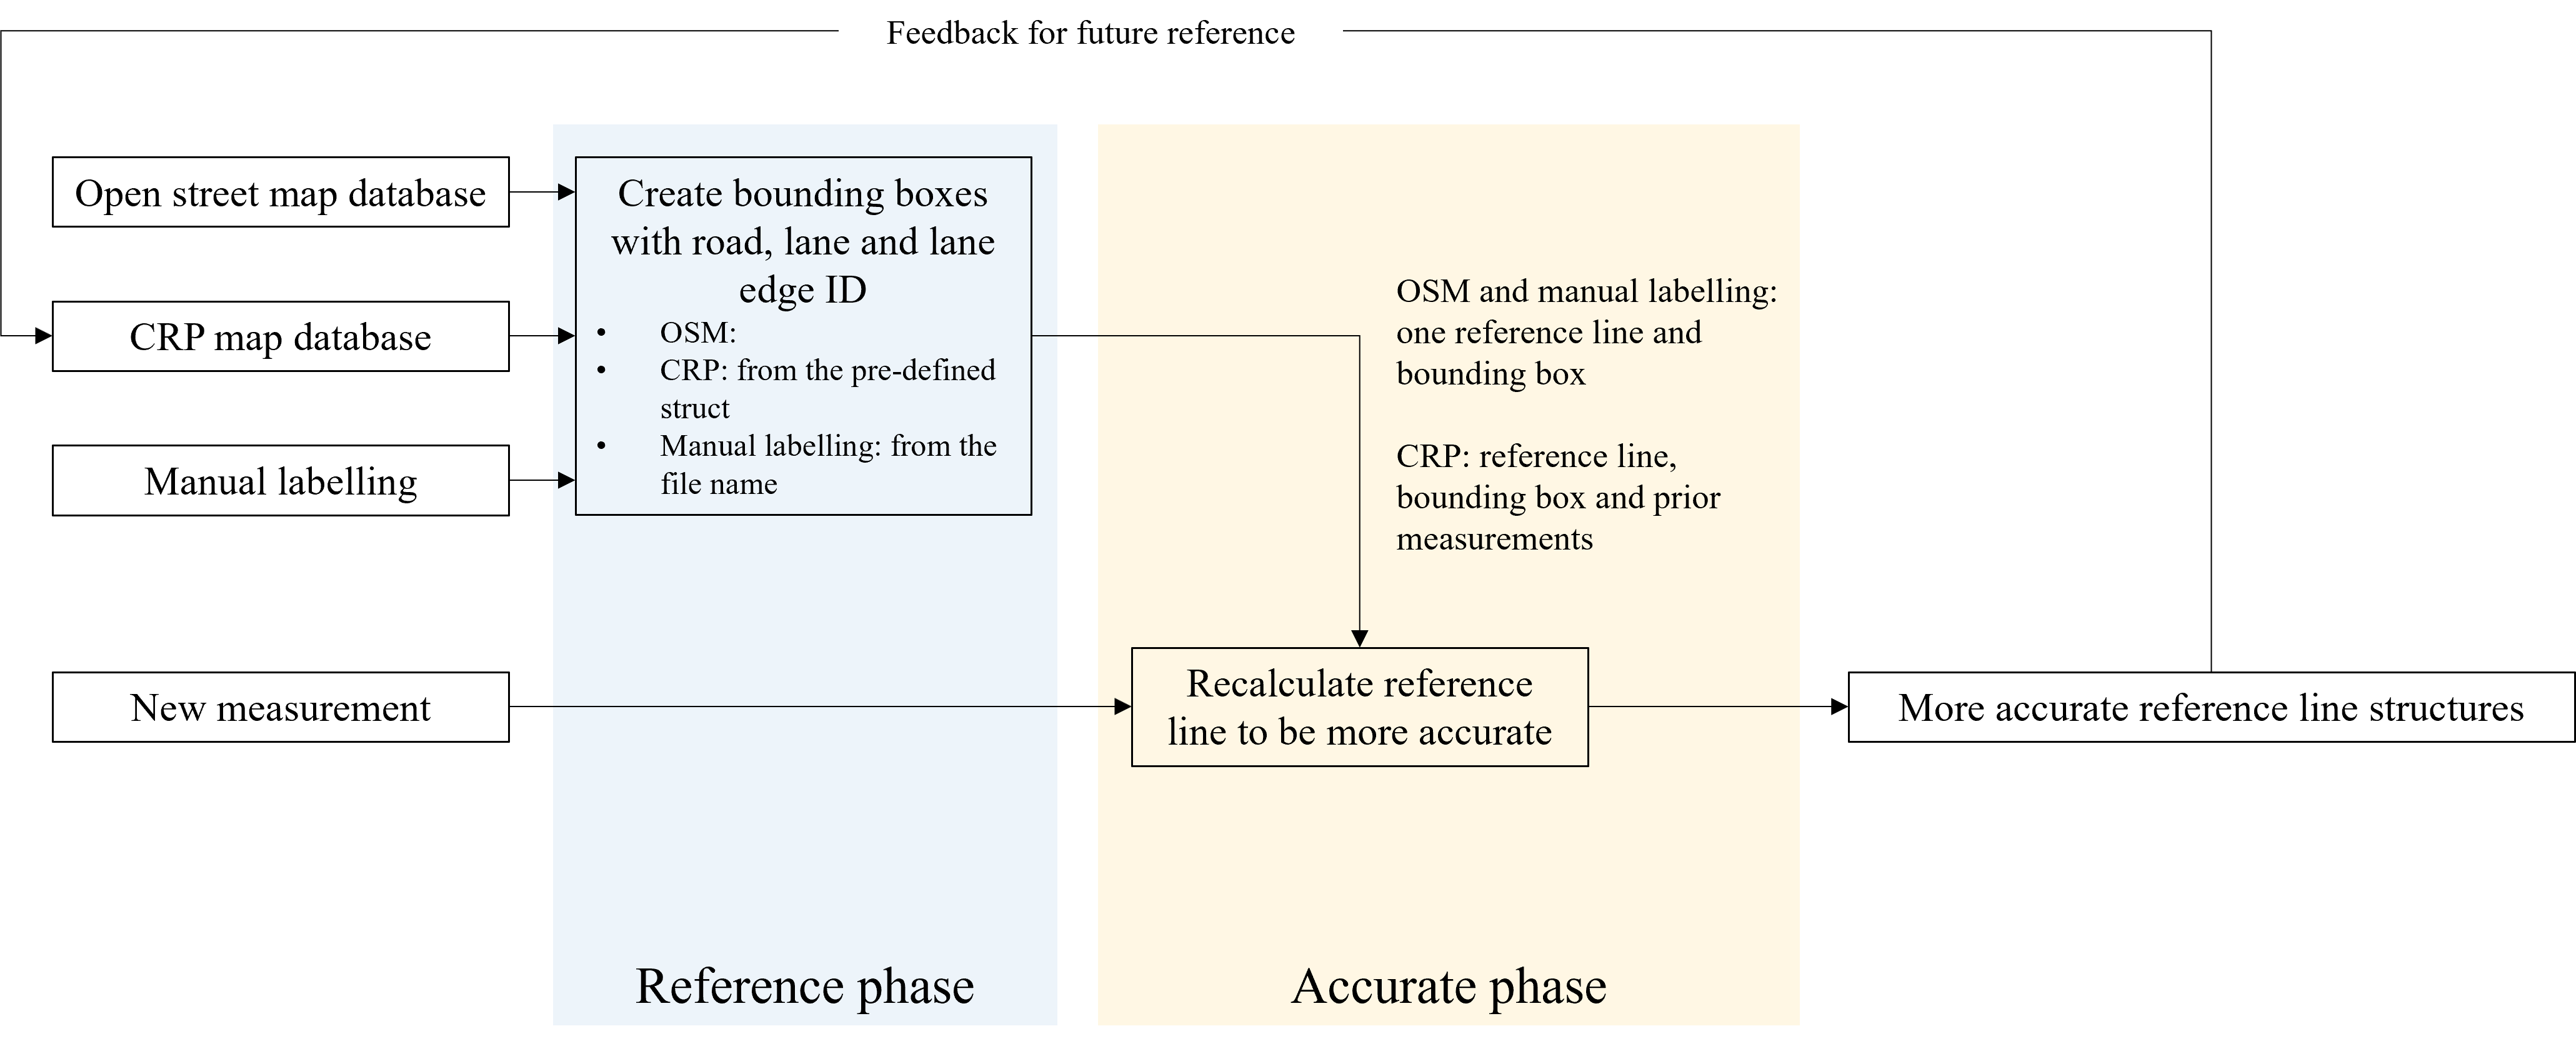
\includegraphics[width=1.0\textwidth]{mapPub/twoPhaseApproach.png}}
    \caption{Two phase approach of reference line creation.}
    \label{fig:twoPhaseApproach}
\end{figure}

\subsection{Manual Reference Phase}
Manual reference lines can be calculated by using own measurements and labelled road and lane id information.
\newline \newline
\fbox{Note: the steps given in this section are implemented in \emph{createManualReference.m}}
\subsubsection{Strictly Monotonic Increasing Coordinates}
The goal is to rotate sections of the route into a frame which provided strictly monotonic increasing X values. This helps to formulate the regression
problem as a function approximation where the $X_{rotated}$ coordinates are the independent variables. Then, a selected function can be fitted.
Even though this is a very 
simple situation, the following procedure can be used in all similar cases, where straight sections are connected via curves:
\begin{itemize}
    \item calculate curvature along the route and cut the route per straights and curves,
    \item rotate snippets to have strictly monotonic X values,
    \item regression of polyline onto the data.
\end{itemize}
Without analytically fitting a curve a telling the curvature based on the curve parameters, numerical derivation can be used.
Nominally, the curvature is the rate of the orientation change, where orientation stands for the tangential direction angle, the rate is calculated based on the step along 
the $X$ axis. In the end, the curvature will be given in $\frac{1}{m}$ unit given the $X$ is in $meters$. The curvature can be calculated per (\ref{eq:curvature}).
\begin{equation} \label{eq:curvature}
    \kappa(t) = \frac{d\Theta}{dX} = \frac{d^2Y}{dX^2}
\end{equation} 
However, the route is given in discrete time, sampled with $T=T_s$ step times. Therefore, (\ref{eq:curvature}) can be rewritten to numerical derivations:
\begin{equation} \label{eq:discrete_orientation}
    \Theta[k] = \frac{Y[k]-Y[k-1]}{X[k]-X[k-1]}
\end{equation}
\begin{equation} \label{eq:discrete_curvature}
    \kappa[k] = \frac{\Theta[k]-\Theta[k-1]}{X[k]-X[k-1]}
\end{equation}
Assuming that $X[k] \neq X[k-1]$. However, in the example shown in Figure \ref{fig:deviation_problem}, this condition is not fulfilled necessarily. Therefore, a pre-check and 
transformation are needed, to ensure that $X$ gets strictly monotonic. Algorithm steps are the following:
\begin{enumerate}
    \item Step 1: calculate mean orientation of the complete route (i.e., $\overline{\Theta} = \frac{1}{N}\sum_{k=1}^{N}\Theta[k]$)
    \item Step 2: rotate the route with $\overline{\Theta}$ and translate it to point $\begin{bmatrix}
        0 & 0 \end{bmatrix}$
    \item Step 3: check, if $X$ is strictly monotonic, if yes, end of algorithm, if no, then continue with Step 4,
    \item Step 4: iterate from the first point along the $X$ axis, until $\abs{X[k]-X[k-1]} \ge dX_{min}$, if not, then Step 5,
    \item Step 5: insert braking point, store previously checked $X-Y$ pairs, reinitialize the checking by repeating Step 3 and Step 4, now with the points deduced by the stored points. Iterate Step 3-5 until the end of the route.
\end{enumerate}
After this algorithm, there are pre-checked snippets, all with strictly monotonic $X$ values, therefore (\ref{eq:discrete_orientation}-\ref{eq:discrete_curvature}) can be calculated for all of them. Then, 
the calculated curvature vectors are concatenated, resulting in the curvature of the original, uncut point series. Now, the following check is done:
\begin{enumerate}
    \item Step 1: find sections, where $\abs{\kappa} < \kappa_{min}$ and label them as straights - $type = 0$,
    \item Step 2: find sections, where $\kappa < -\kappa_{min}$ and label them as right curves - $type = 2$,
    \item Step 3: find sections, where $\kappa > \kappa_{min}$ and label them as left curves - $type = 1$.
\end{enumerate}
Now, given the curve information, the route can be cut into snippets.
\newline \newline
\fbox{Note: the steps given in this subsection are implemented in \emph{calculateRoadCurvatureTypes.m}}

\subsubsection{Bounding Box Creation}
Now, taking the snippets for each reference lanes, a bounding box is calculated which forms a band around the reference line. By using a band, a certain deviation from 
the exact reference line is allowed. This is necessary, as the new measurements must be matched with the reference lines.
\newline \newline
\fbox{Note: the steps given in this subsection are implemented in \emph{createBoundingBoxes.m}}

\subsection{Accurate Phase}
The accurate phase reads in the reference file (from any source), maps the new measurements to the reference lines and make the regression again to yield more accurate 
reference lines.
\newline \newline
\fbox{Note: the steps given in this subsection are implemented in \emph{createMap.m}}

\subsubsection{Regression}
All measurements plotted in the UTM coordinate frame is seen in Figure \ref{fig:ZZ_all}. The circles indicate the starting point of each lines. A few anomalies
are seen:
\begin{itemize}
    \item not all the measurements start at the same localization, there are significant differences for some of them,
    \item there is a deviation between estimated lines due to the aformentioned conditions. These errors are more illustrated in Figure \ref{fig:ZZ_straight_close}.
\end{itemize}
\begin{figure}[h]
    %\captionsetup{justification=raggedleft}
    \center{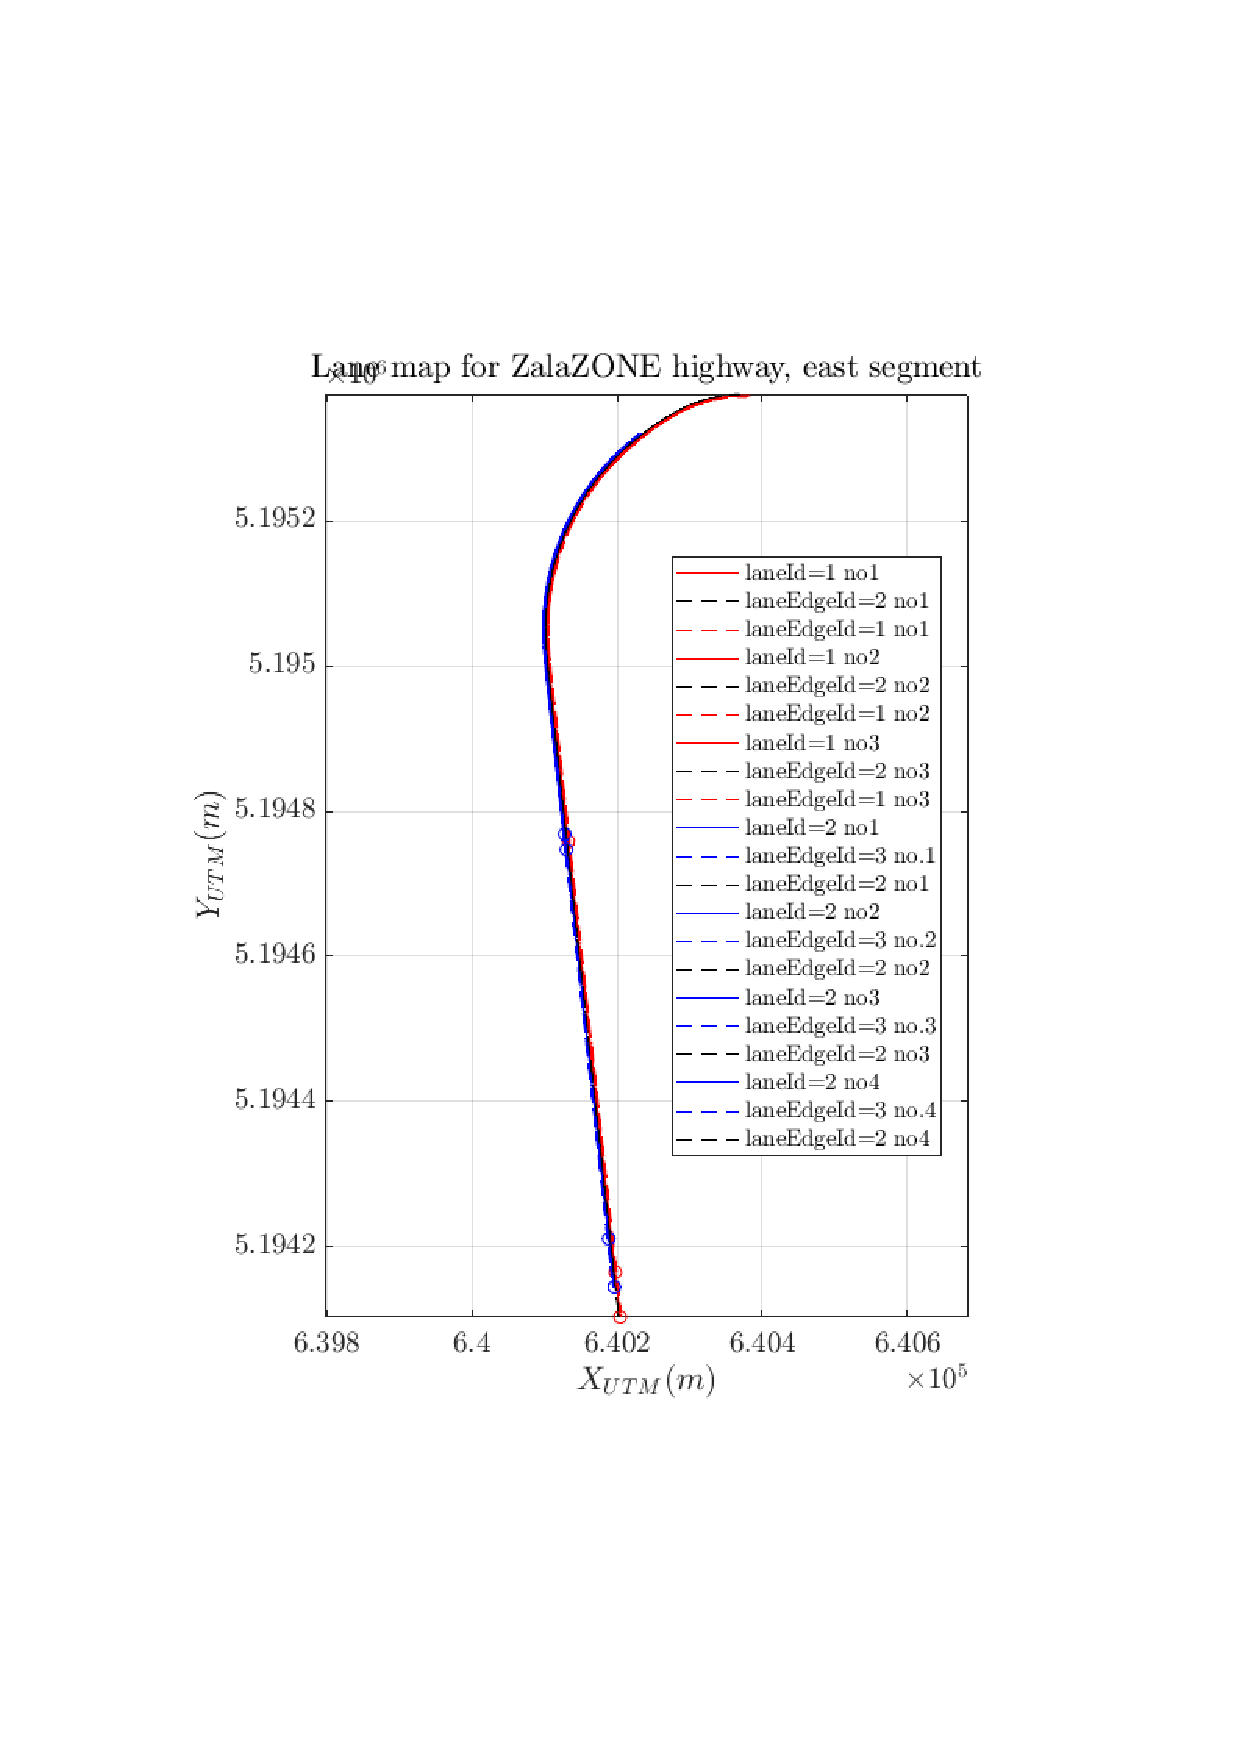
\includegraphics[width=1.0\textwidth]{mapPub/ZZ_all.pdf}}
    \caption{Result of the map data preprocess - sorted lanes from multiple measurement file.}
    \label{fig:ZZ_all}
\end{figure}
\begin{figure}[h]
    %\captionsetup{justification=raggedleft}
    \center{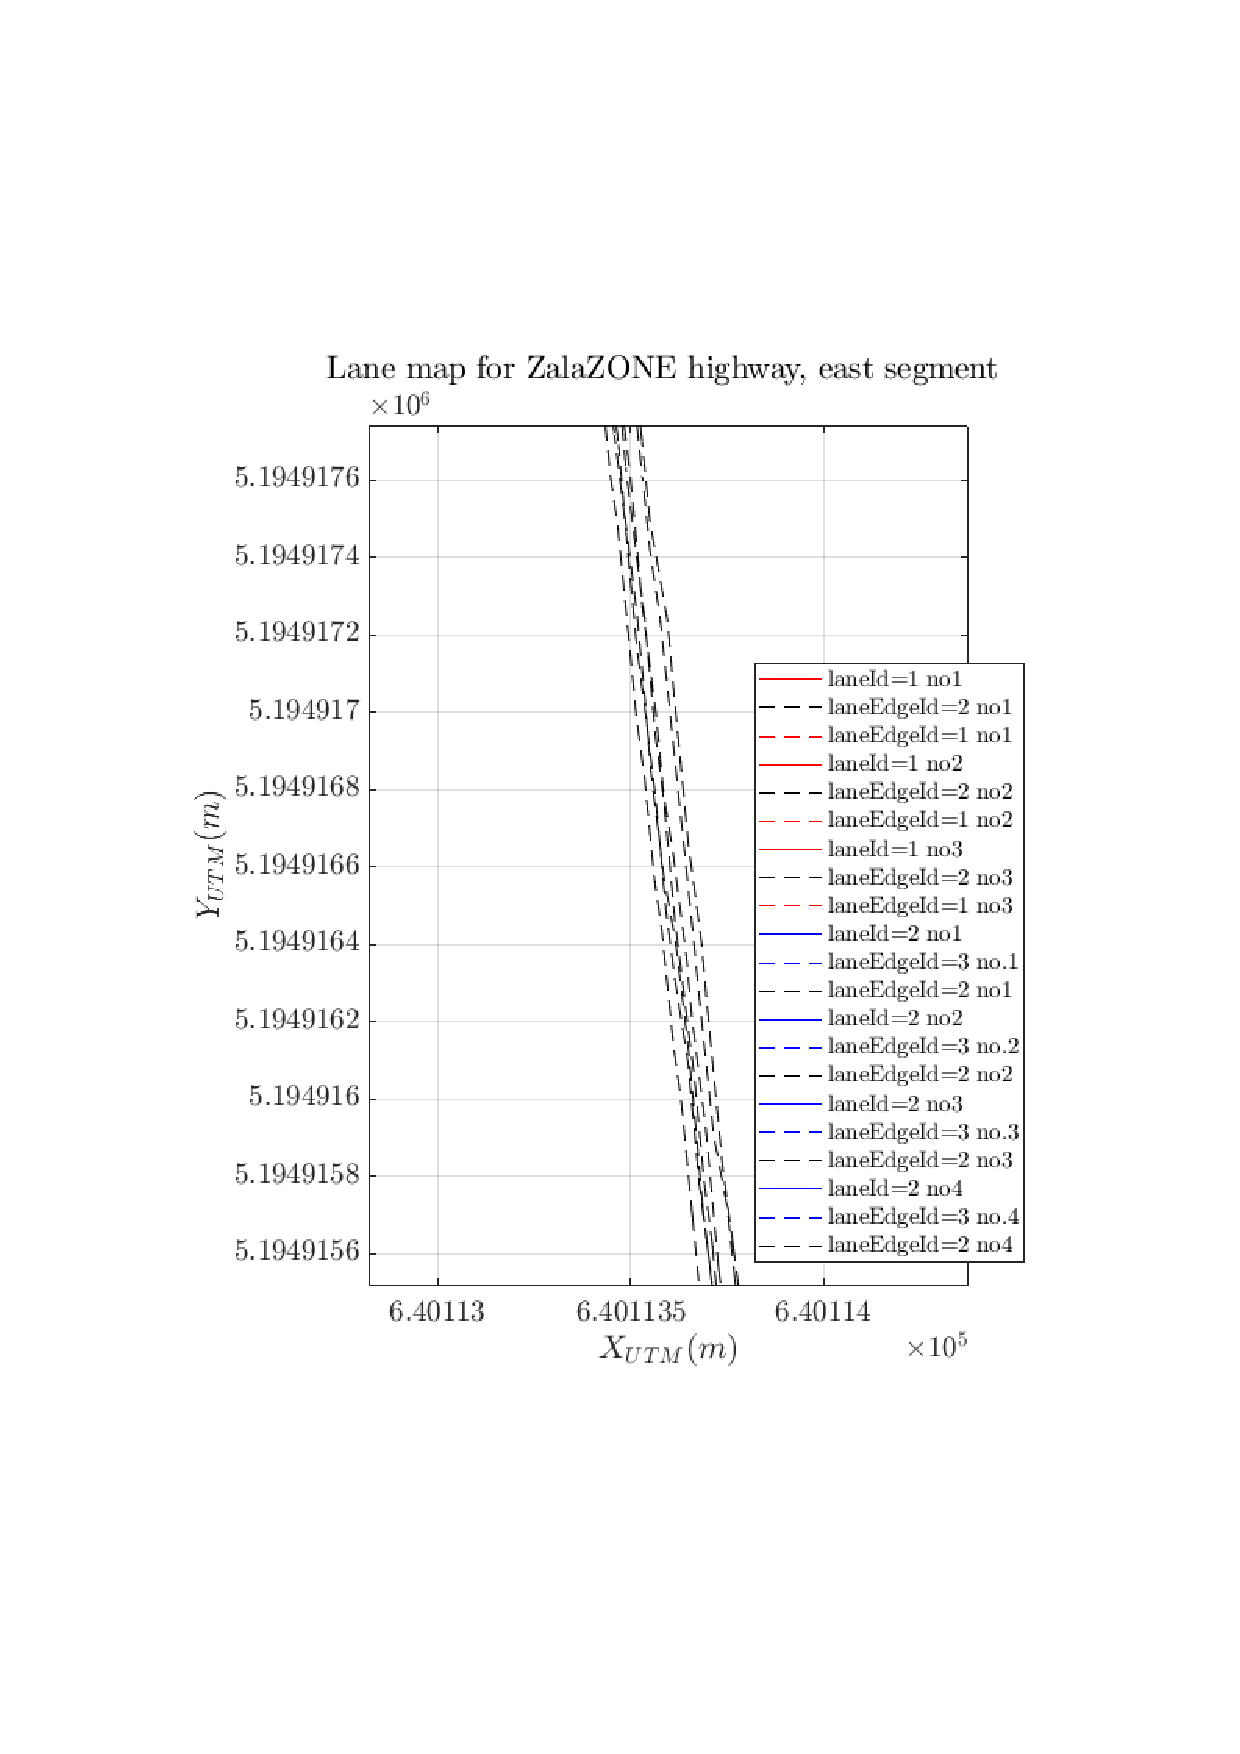
\includegraphics[width=1.0\textwidth]{mapPub/ZZ_straight_mid_close.pdf}}
    \caption{Lane edge id=2. There is a deviation between estimates coming from multiple measurements.}
    \label{fig:ZZ_straight_close}
\end{figure}
Theoretically, the variance of the lane edge estimates can be calculated. However, there are two major issues:
\begin{itemize}
    \item there are not enough measurements to create a probability distribution from point to point,
    \item the points are not sampled at the same position,
    \item orientation of the lane changes between $-\Pi$ and $\Pi$, which may lead to non-monotonic X values, therefore function interpretation is difficult.
\end{itemize}
The second and third problem are illustrated in Figure \ref{fig:deviation_problem}. As during reference phase the snippets are cut to have strictly monotonic 
$X$ local coordinates, the regression problem can be treated as a function approximation problem. 
For example, polylines may be used to describe the lane edge lines. Then, using Least-Square Regression the polyline coefficients can be calculated knowing
the line data ahead. Please be noted that similar solution may be applied when data is not available preliminary (i.e., online estimation), but other techniques, 
such as system identification techniques must be introduced. This increases the complexity of the algorithm and reduced the accuracy. In this case the data 
is available, therefore a full regression can be applied offline, in MATLAB, using preliminary function called \emph{polyfit(x,y,n)} of MATLAB, where $x$ and $y$ are 
vectors of the measurement points, and $n$ is the degree of the polyline. The most important is parameter of the regression is $n$. Choosing a low $n$ saves computational 
time but may lead to poor fit on the data while large value of $n$ results in good fit accuracy but takes more time to calculate and is prone to overfit 
on the data, therefore extrapolation is difficult. The problem can be simplified if the shape of the line to be estimated is simpler, which can be achieved but 
cutting the complete route to snippets. In this case, the route consists of the clearly seen straight section followed by a right curve. 
\begin{figure}[h]
    %\captionsetup{justification=raggedleft}
    \center{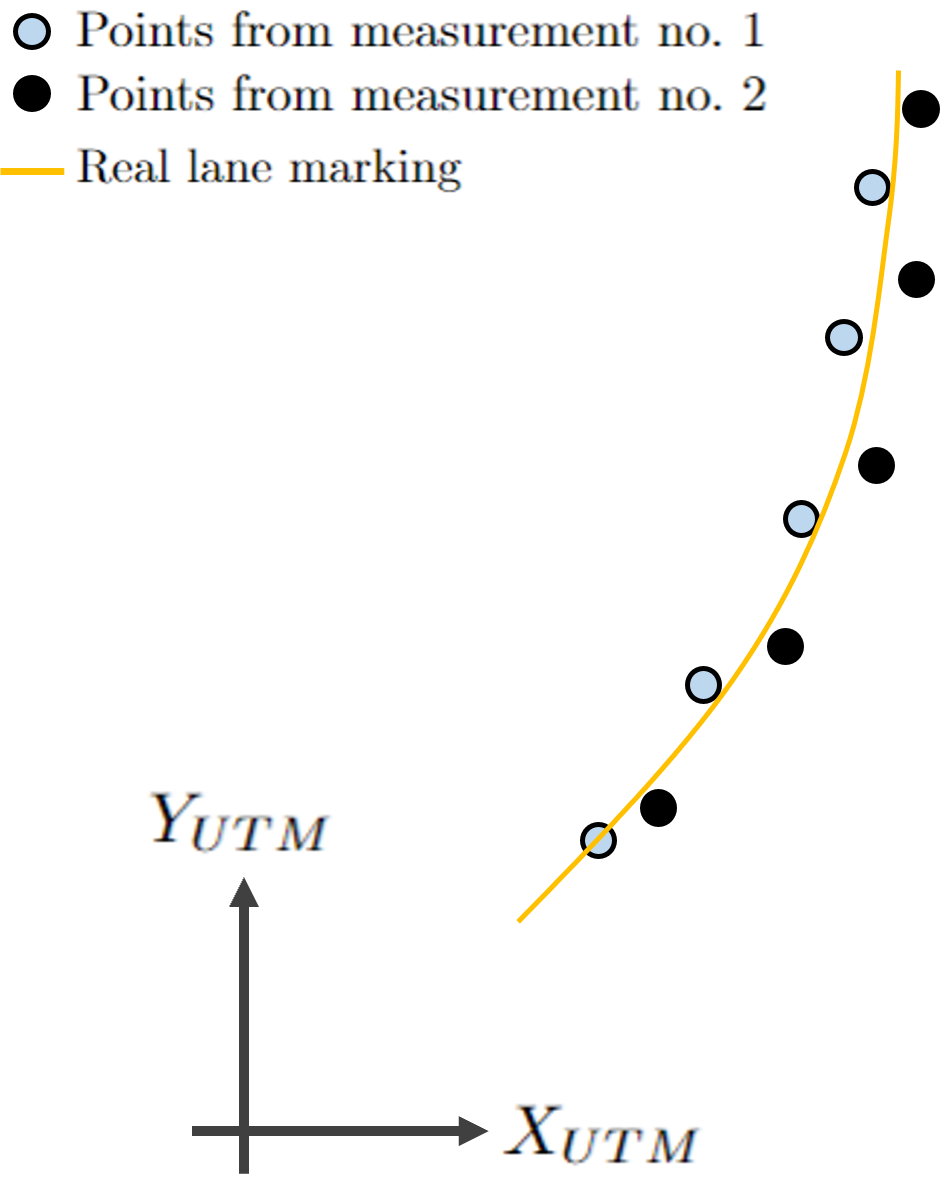
\includegraphics[width=0.6\textwidth]{mapPub/deviation_problem.png}}
    \caption{Illustration of a realistc lane marking detection scenario. Problems are that a) there is a deviation of points due to the localization and 
    detection inaccuracies, and b) the points are given in equal time steps, but without synchronization to each other (measurements are recorded after 
    each other).}
    \label{fig:deviation_problem}
\end{figure}
\newline \newline
\fbox{Note: the steps given in this subsection are implemented in \emph{calculateSmoothLine.m}}

\subsection{Results}
The results are shown in Figure \ref{fig:fittedLines_zoomed}. This is an example, where the original measurement points are shown with small dots, while the regression line is shown as solid.
\begin{figure}[h]
    %\captionsetup{justification=raggedleft}
    \center{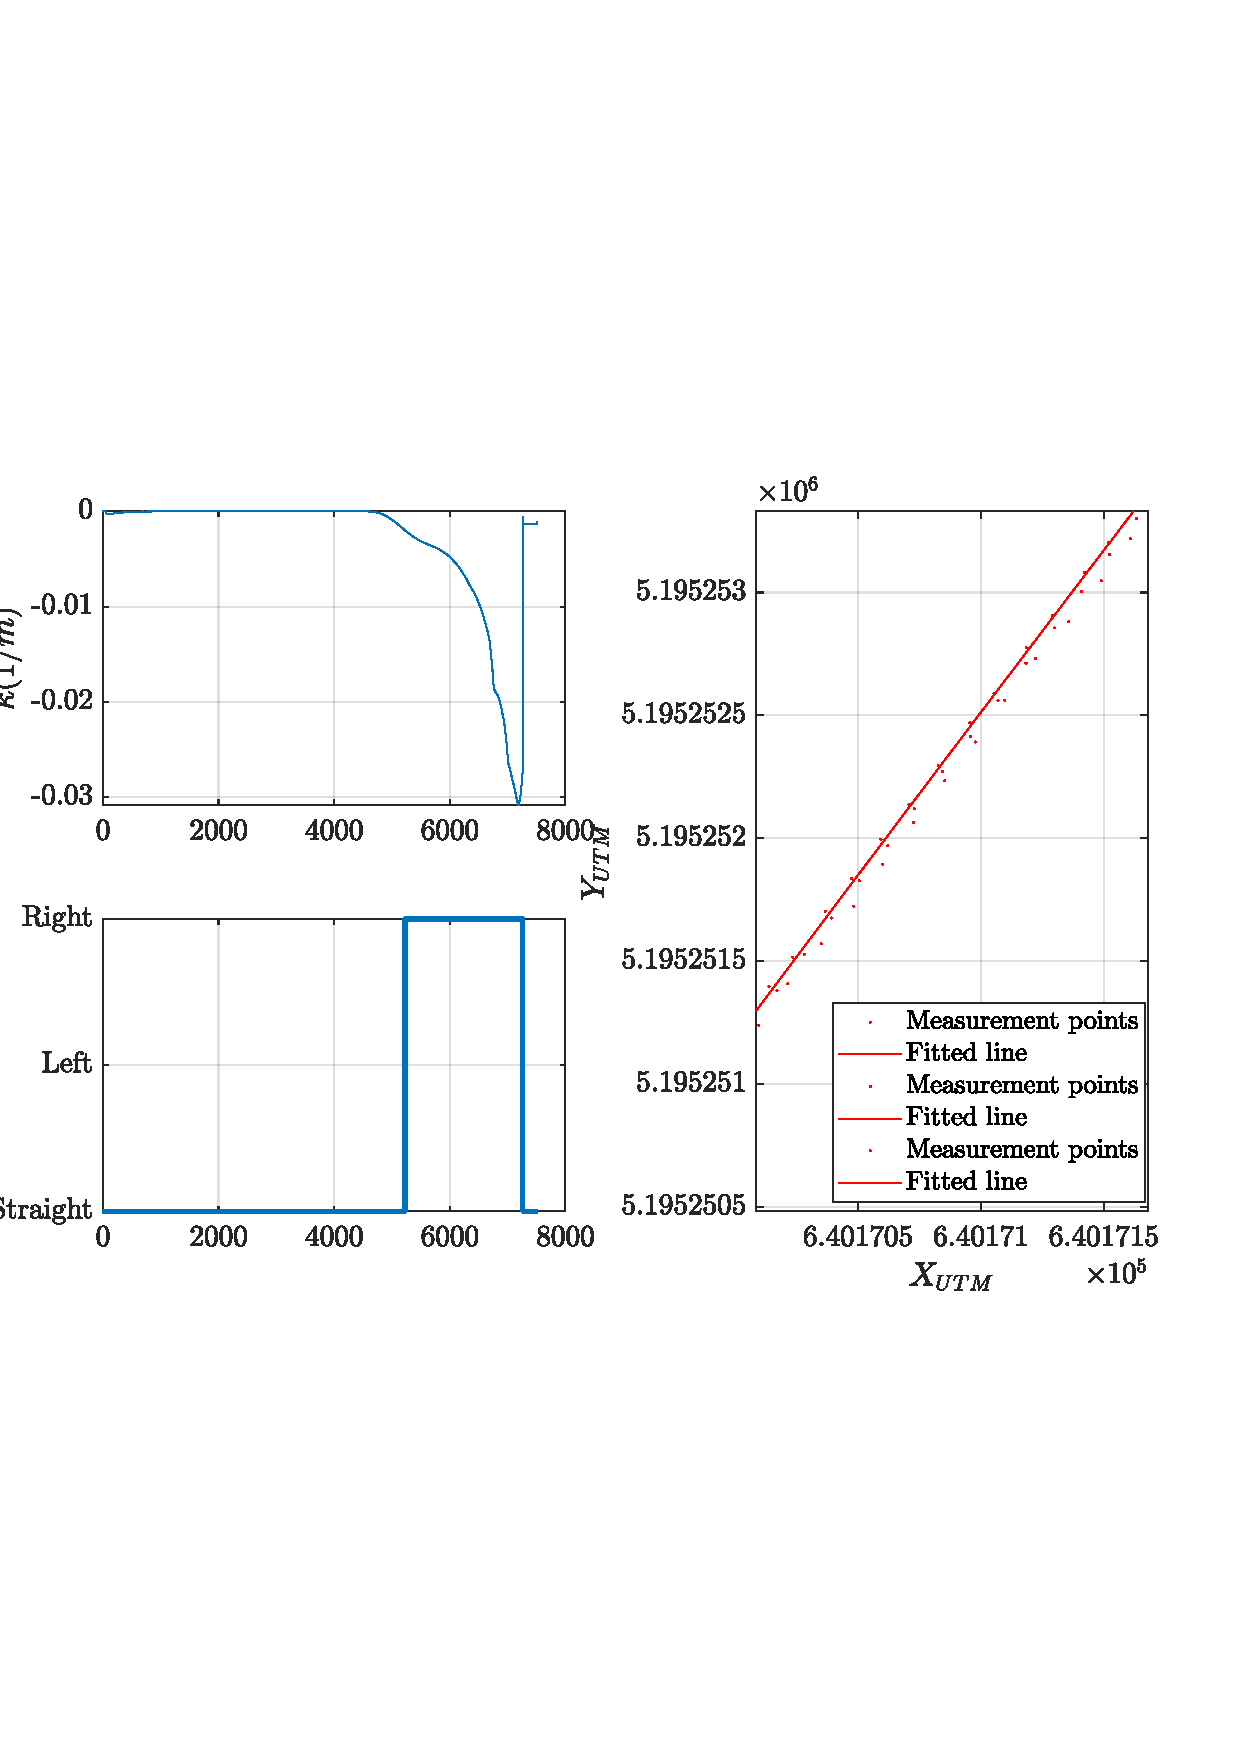
\includegraphics[width=0.6\textwidth]{mapPub/fittedLines_zoomed.pdf}}
    \caption{An example (lane id 1 midlane) of the fitting result. Zoomed in to show the regression performance and make the original measurement points visible.}
    \label{fig:fittedLines_zoomed}
\end{figure}

\begin{figure}[h]
    %\captionsetup{justification=raggedleft}
    \center{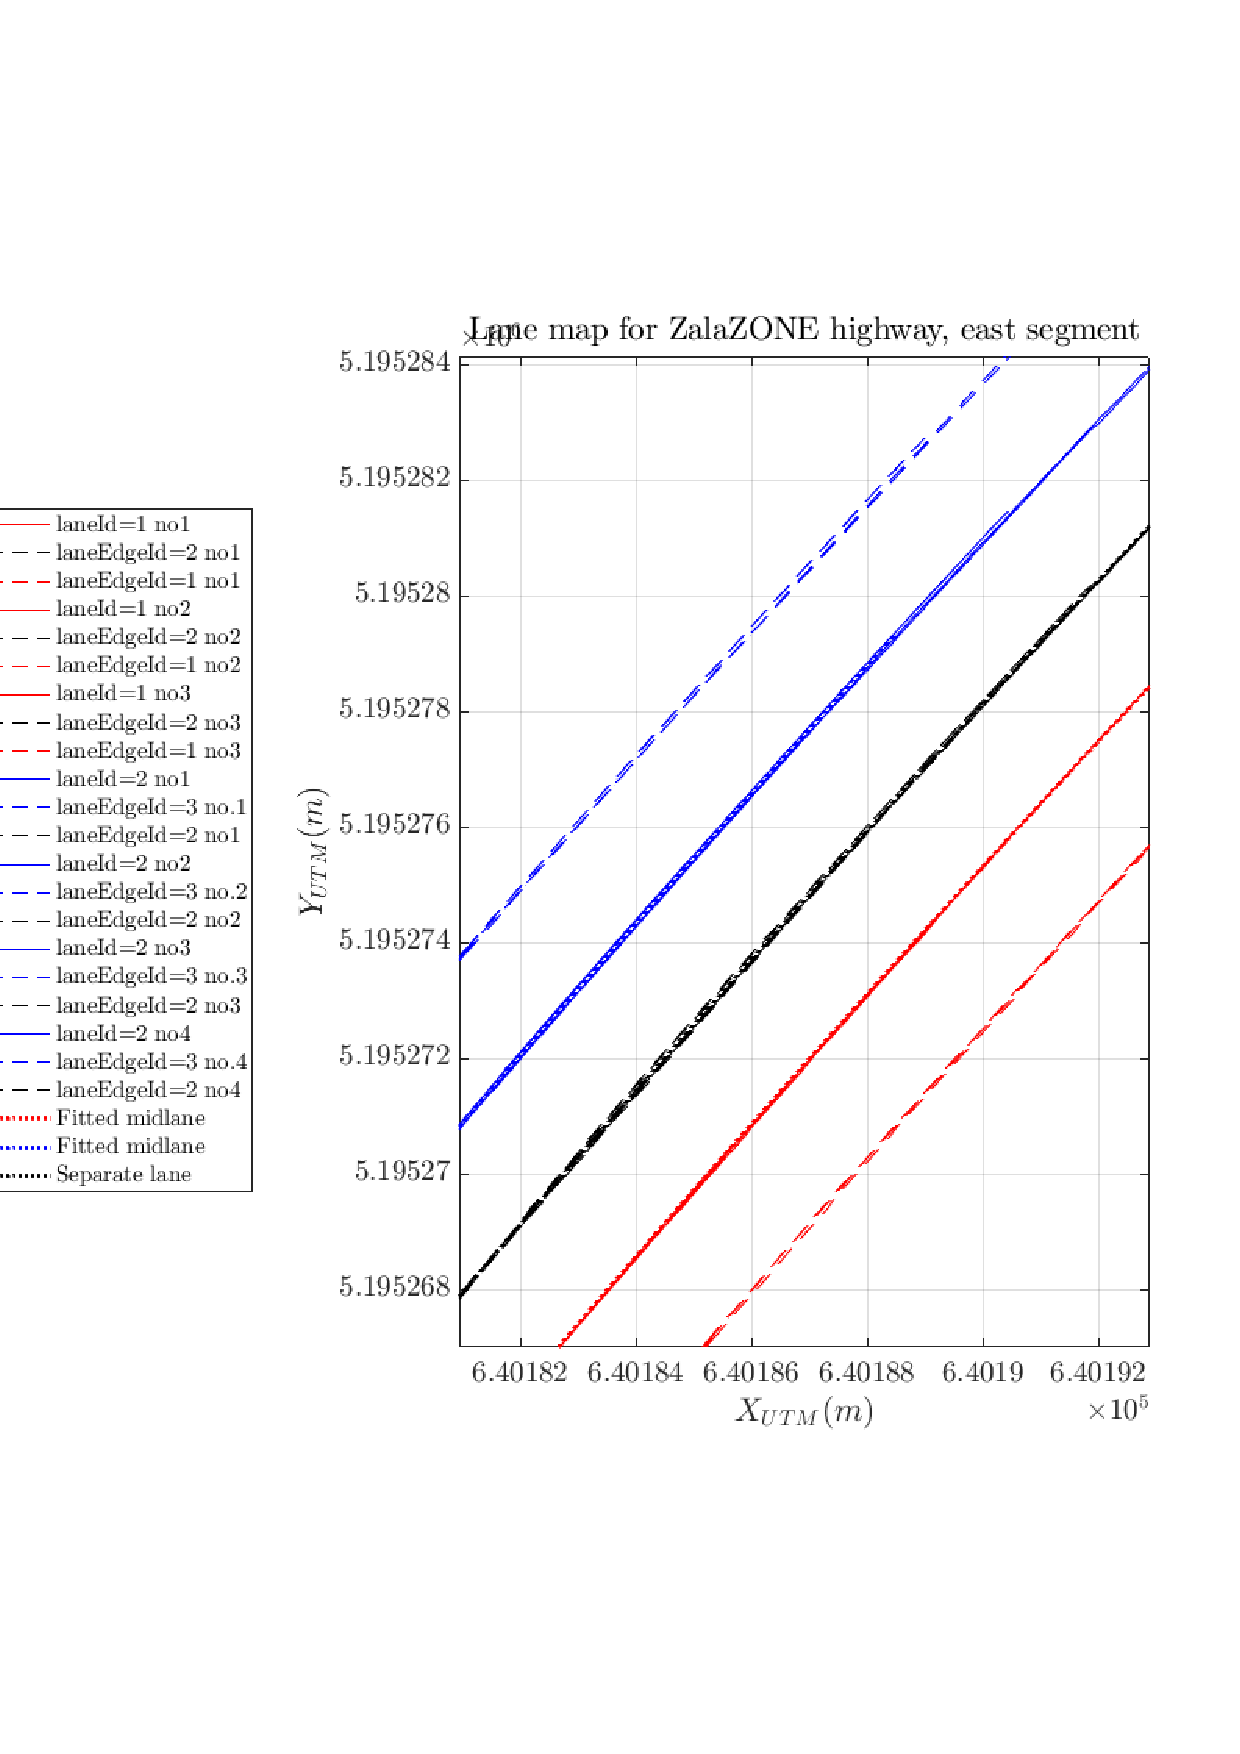
\includegraphics[width=0.6\textwidth]{mapPub/fittedLines.pdf}}
    \caption{Three lines are fitted, and visualized together with the original figure.}
    \label{fig:fittedLines}
\end{figure}

\section{Vehicle Controllers} \label{sec:vehicle_controllers}
\subsection{Compensatory Model} \label{sec:compensatory_model}
The model is based on the combination of various existing models, such as the pure pursuit approach (for the feedforward path) \cite{NovelPP} \cite{MultGoalPP}, the two-point visual control driver model \cite{TwoPoint},
and the compensatory driver model \cite{ContrTheoMod}. The idea is, that there are underlying patterns and the driver acts as a closed loop controller. However, it has been shown that feedforward guess of the target 
road wheel angle (or equal quantity) highly improves the performance. The widely used PID feedback control method, however, often has the bottlenack of being too sensitive on kinematic parameters, especially longitudinal 
velocity. As the connection between the vehicle yawrate and the vehicle curvature is speed dependent, it makes it difficult to directly calculate the target road wheel angle. Furthermore, nonlinearity is increased by 
the geometrical relations between the road wheel angle and the vehicle curvature. Therefore, the problem is divided into three sub-processes:
\begin{itemize}
    \item the tracking controller calculates the lateral acceleration target, which is still linearly connected to the pose error, then
    \item the target lateral acceleration is mapped to the road wheel angle (vehicle curvature), the mapping contains the velocity dependency and geometrical non-linear transformation, then
    \item the road wheel angle (vehicle curvature) is mapped to steering wheel angle (as the actuator control interface provides only steering wheel level communication).
\end{itemize}
The second and third steps are only open-loop mapping of one quantity to another, and the mapping function purely relies on prior, physical assumptions, such as the Ackermann steering equations.
The block diagram of the entire chain is shown in Figure \ref{fig:compensatory_arch}. Please be noted, that the current implementation contains the highly simplified acceleration-to-road-wheel-angle and the road-wheel-angle to 
steering-wheel-angle control maps. 

\begin{figure}[h]
    %\captionsetup{justification=raggedleft}
    \center{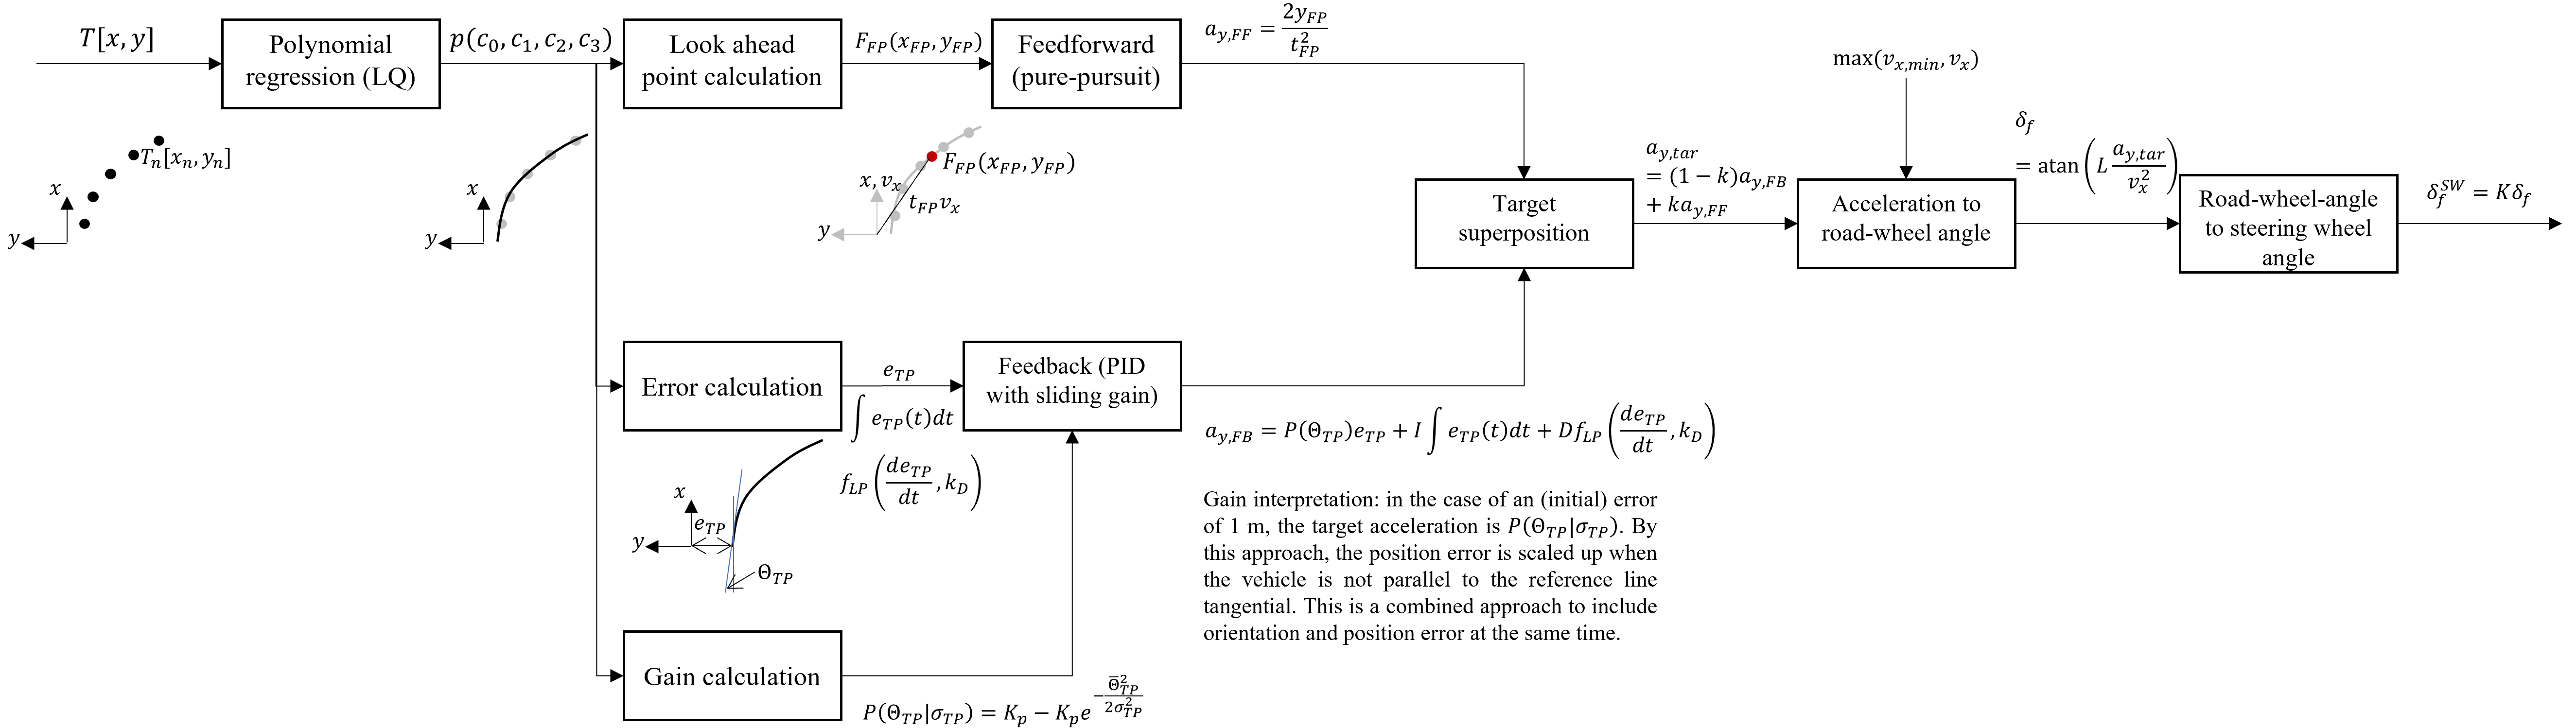
\includegraphics[width=1.0\textwidth]{compensatory_arch.png}}
    \caption{The block diagram of the compensatory driver model.}
    \label{fig:compensatory_arch}
\end{figure}

\bibliography{refs}
\end{document}
